\chapter{Analisis Masalah dan Rancangan Solusi}

Bab ini akan berisikan deskripsi detail terkait persoalan, rencana penyelesaian persoalan, dan solusi yang akan dibangun dalam tugas akhir. Bab ini diharapkan dapat memberikan gambaran jelas pada persoalan yang dibahas dan solusi yang akan dibangun.

% Tujuan utama penulisan bab ini adalah untuk menguraikan rencana penyelesaian masalah tugas akhir I.. Bab ini mencakup antara lain: 
% 1.	Deskripsi dan analisis persoalan yang terkait dengan Rumusan Masalah, misalnya menjelaskan secara detail latar belakang dan masalah yang menjadi dasar munculnya topik, menunjukkan gap/celah antara kondisi saat ini dengan kondisi yang diharapkan, dan kaitan antara sistem/aplikasi yang dikembangkan dengan sistem/aplikasi lain yang terkait.
% 2.	Analisis solusi yang terdiri dari pilihan alternatif solusi yang dapat digunakan untuk setiap permasalahan berdasarkan hasil studi literatur atau survei, pemilihan solusi beserta justifikasinya.
% 3.	Deskripsi umum solusi yang dipilih, mencakup:
% a.	Modul/subsistem/komponen yang akan dikembangkan untuk menyelesaikan masalah, berikut penjelasannya.
% b.	Alur umum algoritma atau langkah-langkah pengembangan sistem dan penjelasannya.
% c.	Penggunaan kakas yang diperlukan
% Dianjurkan untuk menggunakan diagram sebagai pendukung penjelasan bagian ini.

\section{Analisis}

\subsection{Analisis Masalah}
\label{subsec:analisis-masalah}

% Dalam pengembangan dApps, Smart Contracts berperan sebagai \textit{building blocks} yang saling terhubung dan berinteraksi sesuai dengan fungsionalitasnya. Namun, dengan jumlah Smart Contracts yang terus bertambah di blockchain dan ketiadaan mekanisme klasifikasi yang jelas, pemilihan Smart Contracts yang tepat menjadi tantangan yang kompleks. Kesulitan ini terutama muncul dalam pengklasifikasian dan pelabelan Smart Contracts secara semantik, yang berdampak pada sulitnya menemukan Smart Contracts yang sesuai dengan kebutuhan pengguna.

% Kesulitan dalam menemukan Smart Contracts yang sesuai sering kali mendorong pengembang dApps untuk membuat Smart Contracts khusus untuk aplikasi yang dikembangkan, meskipun fungsionalitasnya serupa dengan yang sudah ada. Akibatnya, jumlah Smart Contracts di blockchain tumbuh secara eksponensial, memperbesar ukuran blockchain secara signifikan. Pertumbuhan yang tidak terkendali ini menyebabkan \textit{bloating}, yang berdampak pada inefisiensi penyimpanan dan masalah skalabilitas, sehingga memengaruhi kinerja sistem konsensus. Selain itu, biaya pengembangan dApps pun meningkat karena pengembang harus membuat dan mendeploy Smart Contracts baru untuk setiap aplikasi, meskipun solusi serupa sebenarnya sudah tersedia. Kurangnya dukungan terhadap mekanisme \textit{reusability} ini juga berdampak pada kualitas dari Smart Contracts secara umum karena pengembang cenderung menulis kode yang tidak terjamin secara kualitas.
% terutama dari segi keamanan

% Seringkali butuh untuk berinteraksi dengan kontrak yang udah ada untuk mengakses fungsionalitasnya, ataupun menggunakan sebuah infrastruktur publik
% tapi dengan jumlah SC yang bertambah dan belum ada mekanisme pencarian yang baik, masih sulit untuk mendapatkan SC yang relevan
% Terutama dalam klasifikasinya secara semantik, karena sistem sekarang belum ada, dan kalaupun ada, itu diinput oleh orang yang melakukan verifikasinya saja, yang belum tentu mendeskripsikan dengan sesuai. selain itu, walaupun ada klasifikasi pun, belum ada mekanisme buat menemukan SC yang sesuainya.
Dalam pengembangan Smart Contracts, seringkali dibutuhkan interaksi dengan kontak yang terdapat di blockchain untuk mengakses fungsionalitas kontrak tersebut atau menggunakan sebuah infrastruktur publik. Namun, dengan jumlah Smart Contracts yang terus bertambah dan ketiadaan mekanisma pencarian yang baik, masih sulit untuk mendapatkan Smart Contract yang relevan dengan kebutuhan. Terutama dalam pengklasifikasian Smart Contracts secara semantik yang belum disediakan secara luas oleh sistem-sistem. Sistem yang memiliki mekanisme tersebut seringkali menggunakan mekanisme dimana pengguna yang melakukan pendaftaran Smart Contracts itu sendiri yang memasukkan deskripsi dan kategori dari Smart Contracts, yang belum tentu sesuai dengan kode yang dimiliki kontrak. Selain itu, belum terdapat juga sebuah mekanisme untuk menemukan Smart Contract yang sesuai sehingga sistem klasifikasi yang dimiliki masih belum dapat dimanfaatkan dengan baik.

% Sistem saat ini masih menggunakan sebuah repositori utama untuk mendaftarkan sebuah Smart Contract, sehingga data dari blockchain harus di push ke repositori. Model ini bikin bottleneck karena akan ada banyak instance repositori yang berbeda-beda (contohnya skrg ada Etherscan, Sourcify, untuk mendaftarkan Smart Contract). Di repositori-repositori ini juga belum ada mekanisme pencarian yang baik, karena sekarang masih bersifat lexical, bertumpu pada ketersesuaian kata kunci atau sintaks. Padahal sintaks tidak terlalu merepresentasikan semantik dari sebuah SC.
Sistem-sistem saat ini masih menggunakan pendekatan sebuah repositori utama untuk mendaftarkan Smart Contract, sehingga data dari blockchain harus di-\textit{push} ke repositori oleh masing-masing pengguna. Model ini mengakibatkan \textit{bottleneck} karena akan terdapat banyak \textit{instance} repositori yang berbeda-beda kontennya dengan mekanisme pendaftaran atau verifikasi yang berbeda-beda. Hal ini tercermin dari Etherscan dan Sourcify yang memiliki perbedaan mekanisme untuk mendaftarkan Smart Contracts. Repositori-repositori ini menggunakan mekanisme pencarian berbasis teks ataupun \textit{address} Smart Contracts, yang bersifat leksikal dan bertumpu pada ketersesuaian kata kunci, sintaks, atau \textit{address}. Padahal, sintaks dan \textit{address} tidak dapat merepresentasikan semantik dari Smart Contract dengan baik.

% Karena kesulitan itu, pengembangan sistem SC sering terhambat, seperti hambatan dalam mencari kontrak untuk mengintegrasikan dengan USDC, sebuah stablecoin yang umum, di tengah banyaknya kontrak fraud. atau contoh lainnya adalah menggunakan router decentralized exchange seperti uniswap atau sushiswap.
% Selain menggunkana instance, ada juga kontrak yang emang di deploy sebagai infrastructure publik seperti Uniswap V3 Factory, atau ENS registry, oracles, bridges, etc
Kesulitan-kesulitan itu menghambat pengembangan sistem Smart Contracts, seperti hambatan dalam pencarian kontrak untuk mengintegrasikan USDC, sebuah \textit{stablecoin} yang umum, di tengah banyaknya kontrak \textit{fraud}; atau hambatan dalam mencari \textit{router} untuk \textit{Decentralized Exchange} seperti UniSwap atau SushiSwap. \textit{Use case} lainnya untuk penggunaan ulang ini adalah kontrak yang berperan sebagai infrastruktur publik, seperti UniSwap V3 Factory, ENS Registry, Oracles, Bridges, dan lainnya.

% Banyak penelitian yang udah mencoba menjawab permasalahan ini, untuk bridge the gap antar kebutuhan dengan semantik dari apa yang dikerjakan oleh kontrak secara nyata, dan salah satu approach nya adalah dengan menggunakan AI untuk mendeskripsikan semantik yaitu fungsi dan maksud dari sebuah Smart Contracts (insert citations), tapi masalahnya adalah riset ini tidak open source, tidak ada data pipeline untuk mengintegrasikan menjadi sistem yang dapat digunakan di industri, dan masih menggunakan model lama.
Terdapat banyak penelitian yang sudah mencoba menjawab permasalahan ini, yaitu untuk menjembatani kesenjangan antar kebutuhan pengguna dengan semantik dari apa yang sebenarnya terjadi di dalam sebuah kontrak. Salah satu pendekatan untuk menyelesaikan permasalahan ini adalah menggunakan AI untuk mendeskripsikan semantik yaitu fungsi dan maksud dari sebuah Smart Contracts \parencite{zhang2021smart} \parencite{stan} \parencite{shi2021semantic} \parencite{shi2021semantic}. Permasalahan dari riset-riset ini adalah kesenjangan antar konsep yang ditawarkan dengan \textit{use case} dan posisi dengan industri karena sistem yang ditawarkan tidak bersifat terbuka dan tidak terdapat sebuah \textit{pipeline} yang dapat digunakan di industri yang mengintegrasikan data blockchains eara langsung. Selain itu, riset-riset ini juga belum mengeksplorasi kapabilitas model-model LLM modern untuk mengerti dan menganalisis semantik dari sebuah kode.

\subsubsection{Dekomposisi Masalah}
\label{subsubsec:dekomposisi-masalah}
% masalah utama: sulit untuk menemukan Smart Contracts yang sesuai dengan kebutuhan pengguna di tengah banyaknya Smart Contracts yang ada pada Blockchain. Kesulitan ini terutama muncul dalam pengklasifikasian dan pelabelan Smart Contracts secara semantik, yang berdampak pada sulitnya menemukan Smart Contracts yang sesuai dengan kebutuhan pengguna.
% dampak masalah: pertumbuhan jumlah Smart Contracts yang tidak terkendali dan peningkatan ukuran Blockchain (\textit{bloating}), peningkatan biaya dan waktu serta penurunan kualitas karena kurangnya mekanisme \textit{reusability} Smart Contracts.

% dekomposisi permasalahan
% 1. bagaimana mengekstraksi data smart contracts dari Blockchain
% 2. bagaimana menyimpan dan mengelola data smart contracts yang sudah diekstrak
% 3. (ini nanti jawabannya dengen semantik enrichment) bagaimana melabelkan dan mengklasifikasikan Smart Contracts yang akan mempermudah pencarian berdasarkan kebutuhan pengguna -> untuk identifikasi kebutuhan yang dijawab oleh Smart Contract
% 4. bagaimana melakukan manajemen terhadap data smart contracts yang sudah dilabelkan dan diklasifikasikan
% 5. (ini nanti jawabannya pake RAG) bagaimana menghubungkan permintaan kebutuhan pengguna dengan data yang sudah dilabelkan dan diklasifikasikan

Secara singkat, masalah utama yang diidentifikasi adalah kesulitan untuk menemukan Smart Contracts yang sesuai dengan kebutuhan pengguna. Masalah ini terutama muncul karena ketiadaan mekanisme klasifikasi yang jelas untuk mengidentifikasi Smart Contracts dan mekanisme pencarian Smart Contracts yang dapat mengakomodasi klasifikasi tersebut.

Permasalahan ini dapat dijawab dengan sebuah mekanisme pencarian Smart Contracts yang lebih akurat dan efisien, yang memungkinkan pengguna untuk menemukan Smart Contracts yang sesuai dengan kebutuhan mereka dengan memanfaatkan pelabelan atau pengklasifikasian dari Smart Contracts. Mekanisme ini juga diinspirasi oleh gabungan dari Semantic Web dan blockchain seperti pada GraphChain \parencite{sopek2018graphchain}, yang memungkinkan untuk melakukan pencarian Smart Contracts berdasarkan semantik yang lebih mendalam. Dengan demikian, pengguna dapat menemukan Smart Contracts yang sesuai dengan kebutuhan mereka dengan lebih mudah dan efisien.
% berdasarkan kebutuhan yang dijawabnya

% ini masih umum kaya yaudah ini idenya dan emang cara solve nya ini, tapi nanti di bab berikutnya itu fokusnya gimana implementasinya dan ide utama yang menawarkan kebaruannya tuh apa

Untuk mengembangkan mekanisme tersebut, digunakan referensi dengan kasus serupa, yaitu Data Retrieval Pipeline yang digunakan dalam RAG \parencite{CrateDB_RAG_Pipelines}. Referensi ini dipilih karena pada dasarnya mekanisme yang akan dikembangkan merupakan Data Retrieval Pipeline. Berdasarkan referensi tersebut, terdapat beberapa poin penting yang perlu dijawab, dan poin-poin ini akan menjadi dasar pemilihan teknologi serta metode yang digunakan dalam sistem yang akan dibangun. Berikut adalah poin-poin dekomposisi masalah yang menjadi dasar tugas akhir ini:

\begin{enumerate}
	\item Bagaimana melakukan ekstraksi data Smart Contracts dari blockchain?

	\item Bagaimana menyimpan dan mengelola data Smart Contracts yang sudah diekstrak?

	\item Bagaimana melabelkan atau mengklasifikasikan Smart Contracts yang akan mempermudah pencarian berdasarkan kebutuhan?

	\item Bagaimana melakukan manajemen terhadap data Smart Contracts yang sudah dilabelkan dan diklasifikasikan?

	\item Bagaimana memahami kebutuhan dari pengguna?

	\item Bagaimana menghubungkan permintaan kebutuhan pengguna dengan data yang sudah dilabelkan dan diklasifikasikan?

	\item Bagaimana melakukan pencarian dan memfasilitasi penggunaan ulang tanpa mempengaruhi kinerja sistem?

	\item Bagaimana mempermudah integrasi Smart Contracts dalam pengembangan dApps?
\end{enumerate}

% \subsubsection{Dampak Masalah}
\label{subsubsec:dampak-masalah}

Secara lebih luas, dampak dari permasalahan utama yang telah diidentifikasi adalah:

\begin{enumerate}
	\item \textbf{\textit{Codebase} yang Kompleks} \newline
	      Redundansi pengembangan Smart Contracts menghasilkan \textit{codebase} yang tumbuh besar dan semakin sulit untuk dipelihara. Kompleksitas ini dapat dihindari jika pengembang mampu menggunakan kembali Smart Contracts yang sudah ada, sehingga efisiensi pengelolaan kode meningkat.
	\item \textbf{Keterbatasan Pengembangan Sistem} \newline
	      Lingkungan pengembangan Smart Contracts yang saat ini sudah mendukung arsitektur berbasis Service-Oriented Architecture (SOA) atau Object-Oriented Approach (OOA) menjadi kurang optimal, karena pengembang lebih banyak berfokus pada pembuatan kontrak baru daripada memanfaatkan kembali kontrak yang sudah ada. Hal ini membatasi potensi inovasi pengembangan internal dApps.
	\item \textbf{Biaya dan Waktu Pengembangan yang Tinggi} \newline
	      Membuat dan mendeploy Smart Contracts baru membutuhkan biaya signifikan, termasuk biaya \textit{deployment} ke jaringan blockchain, yang semakin besar dengan frekuensi pengembangan yang tinggi. Selain itu, waktu yang dihabiskan untuk membuat kontrak baru juga meningkat, memperlambat proses pengembangan aplikasi secara keseluruhan.
	\item \textbf{Inefisiensi Blockchain} \newline
	      Dengan sifat blockchain sebagai ledger terdistribusi, setiap Smart Contract yang di-\textit{deploy} akan tetap tersimpan secara permanen. Redundansi kontrak ini memperbesar ukuran blockchain, memperlambat akses data, dan menciptakan \textit{bottleneck} yang mengurangi efisiensi sistem secara keseluruhan. Masalah ini tidak hanya berdampak pada penyimpanan, tetapi juga memengaruhi kemampuan blockchain untuk mendukung aplikasi berskala besar.
	\item \textbf{Kerentanan Keamanan} \newline
	      Semakin banyak baris kode yang ditulis, akan semakin besar kemungkinan terdapat kerentanan. Dengan kurangnya prinsip \textit{reusability}, banyak kode yang ditulis kembali tetapi tidak terjamin secara kualitas, sehingga meningkatkan risiko kesalahan dan kerentanan keamanan yang mungkin terjadi.
\end{enumerate}

\subsubsection{Kebutuhan Utama}
\label{subsubsec:kebutuhan-utama}

Berdasarkan permasalahan utama dan dekomposisi masalah yang sudah diidentifikasi, muncul beberapa kebutuhan utama untuk menyelesaikannya, terutama yang berkaitan dengan pengelolaan dan penggunaan Smart Contracts. Berikut adalah beberapa kebutuhan yang perlu dijawab:

% \begin{enumerate}
%   \item \textbf{Peningkatan \textit{Reusability} Smart Contracts} \newline
%   Dibutuhkan sebuah sistem yang dapat meningkatkan \textit{reusability} dari Smart Contracts yang sudah ada. Hal ini penting untuk mengurangi redundansi dalam pengembangan Smart Contracts baru yang sebenarnya memiliki fungsionalitas serupa. Dengan adanya mekanisme pencarian berdasarkan fungsionalitas dan semantik, pengembang dapat memanfaatkan kontrak yang tersedia tanpa perlu menulis dari awal, sehingga menekan biaya serta waktu \textit{deployment}.
%   \item \textbf{Manajemen \textit{Smart Contracts} yang Efisien} \newline
%   Dibutuhkan sistem yang mendukung manajemen Smart Contracts secara efisien. Sistem ini tidak hanya membantu dalam melakukan pelabelan dan pengklasifikasian Smart Contracts berdasarkan fungsinya, tetapi juga memungkinkan pengembang untuk memahami hubungan antar kontrak. Dengan pendekatan manajemen yang baik, proses pengelolaan Smart Contracts menjadi lebih terstruktur dan sistematis, yang pada akhirnya memudahkan integrasi dalam pengembangan dApps.
%   \item \textbf{Solusi \textit{Off-Chain} untuk Mengurangi Beban Blockchain} \newline
%   Untuk mengurangi beban pada Blockchain, diperlukan solusi yang memungkinkan sebagian proses dilakukan di luar jaringan Blockchain (off-chain). Dengan cara ini, pencarian dan pengelolaan Smart Contracts dapat dilakukan tanpa membebani kapasitas penyimpanan atau mengganggu efisiensi sistem konsensus di Blockchain. Solusi semacam ini dapat menjadi pendukung utama untuk menciptakan ekosistem Blockchain yang lebih skalabel dan efisien.
%   \item \textbf{Pengurangan Biaya dan Waktu Pengembangan} \newline
%   Selain meminimalkan redundansi, sistem yang dikembangkan harus membantu menekan biaya dan waktu pengembangan. Dengan menyediakan mekanisme pencarian berbasis semantik yang tepat sasaran, pengembang dapat langsung menemukan dan menggunakan Smart Contracts yang sudah ada, menghemat biaya \textit{deployment} baru dan waktu pengembangan.
%   \item \textbf{Skalabilitas dan Efisiensi Penyimpanan Blockchain} \newline
%   Solusi yang diusulkan juga harus mendukung peningkatan skalabilitas dan efisiensi penyimpanan Blockchain. Dengan mengurangi jumlah Smart Contracts yang \textit{redundant}, sistem ini dapat membantu mencegah \textit{bloating} Blockchain dan memastikan penyimpanan tetap efisien, sehingga jaringan dapat terus mendukung pengembangan aplikasi berskala besar.
% \end{enumerate}

% kebutuhan yang muncul
% 1. sistem harus bisa klasifikasi fungsional dan semantik dari sc (semantic enrichment)
% 2. import dan reuse sc harus dipermudah oleh sistem || sistem harus bisa memudahkan reusability -> lebih mudah untuk reuse sc
% 3. sistem harus bisa manajemen sc -> grouping sc berdasarkan label semantik
% 4. sistem harus berjalan secara offchain -> tidak membebani blockchain

% 5. sistem harus bisa ekstraksi data sc dari blockchain
% 6. sistem harus bisa menyimpan dan mengelola data sc yang sudah diekstrak
% 7. sistem harus bisa mentranslasikan kebutuhan pengguna ke query yang sesuai
% 8. data yang disimpan di dalam sistem harus dapat dilakukan query 

\begin{enumerate}
	\item \textbf{Kebutuhan Ekstraksi Data Smart Contracts (K1)} \newline
	      Sistem harus mampu mengekstraksi data Smart Contracts yang ada di Blockchain untuk dapat diproses dan digunakan lebih lanjut.
	      % DK1

	\item \textbf{Kebutuhan Penyimpanan dan Pengelolaan Data Smart Contracts (K2)} \newline
	      Sistem harus dapat menyimpan dan mengelola data Smart Contracts yang telah diekstrak dan di-\textit{enrich}, sehingga data dapat diakses dan digunakan untuk pencarian lebih lanjut.
	      % DK2, DK4

	\item \textbf{Kebutuhan Klasifikasi Fungsional dan Semantik (K3)} \newline
	      Sistem harus dapat mengklasifikasikan Smart Contracts berdasarkan fungsionalitas dan semantik, dengan memperkaya data semantik (\textit{semantic enrichment}) untuk memudahkan pencarian kontrak yang relevan.
	      % DK3, DK5

	\item \textbf{Kebutuhan Solusi \textit{Off-Chain} (K4)} \newline
	      Sistem harus berjalan secara \textit{off-chain} untuk mengurangi beban pada jaringan Blockchain dan meningkatkan skalabilitas.
	      % DK7

	\item \textbf{Kebutuhan Translasi Kebutuhan Pengguna ke Smart Contracts (K5)} \newline
	      Sistem harus dapat mentranslasikan kebutuhan fungsionalitas yang diajukan oleh pengguna menjadi kontrak yang relevan.
	      % DK5, DK6 

	\item \textbf{Kebutuhan Kemampuan Query Data (K6)} \newline
	      Data yang disimpan dalam sistem harus dapat di-query dengan mudah untuk memungkinkan pengambilan informasi yang relevan.
	      % DK6

	\item \textbf{Kebutuhan Peningkatan \textit{Reusability} (K7)} \newline
	      Sistem harus memudahkan penggunaan ulang Smart Contracts yang telah ada, dengan memastikan kemudahan dalam melakukan \textit{import} Smart Contract.
	      % DK8
\end{enumerate}

Kebutuhan-kebutuhan ini akan menjadi dasar dalam merancang solusi yang tepat untuk mengatasi permasalahan utama yang diidentifikasi sebelumnya. Dengan memenuhi kebutuhan-kebutuhan tersebut, diharapkan solusi yang diusulkan dapat memberikan manfaat yang maksimal bagi pengguna dalam mengelola dan menggunakan Smart Contracts di Blockchain.

% Bisa dikasih visualisasi juga 

% \subsubsection{Ajuan Solusi}
\label{subsubsec:ajuan-solusi}

Berdasarkan kebutuhan-kebutuhan utama yang telah diidentifikasi, diperlukan sebuah solusi yang mampu menjawab berbagai tantangan dalam pengelolaan dan penggunaan Smart Contracts di blockchain. Solusi ini harus memungkinkan pencarian Smart Contracts berdasarkan fungsionalitasnya, sehingga pengembang tidak perlu membuat kontrak baru setiap kali mengembangkan dApps, terutama ketika kontrak dengan fungsionalitas serupa sudah tersedia. Dengan meningkatkan \textit{reusability} dari Smart Contracts yang ada, sistem ini dapat membantu menekan redundansi dan mengoptimalkan penggunaan sumber daya yang ada.

Untuk memenuhi kebutuhan ini, diajukan sebuah sistem pencarian Smart Contracts berbasis semantik yang dirancang untuk:

% rancangan solusi
% 

\begin{enumerate}
	\item Mengidentifikasi Smart Contracts dengan fungsionalitas yang sesuai berdasarkan kebutuhan pengembang. (AS1)
	\item Merekomendasikan Smart Contracts yang sudah ada dengan mempertimbangkan hubungan semantik antar kontrak, sehingga hasil pencarian lebih relevan dan dapat langsung digunakan. (AS2)
	\item Mendukung efisiensi biaya, waktu, dan pengelolaan blockchain, dengan memastikan bahwa proses pencarian dan pengelolaan dilakukan secara terstruktur dan tidak membebani jaringan blockchain. (AS3)
	      % tidak membebani dengan cara off-chain -> melakukan ekstraksi di luar blockchain, mapping di luar blockchain dst
	\item Merekomendasikan Smart Contracts yang aman dan terpercaya dengan mempertimbangkan verifikasi dari Smart Contracts. (AS4)
\end{enumerate}

Solusi ini dirancang untuk memenuhi kebutuhan \textit{reusability}, manajemen Smart Contracts, dan efisiensi sistem, sekaligus mendukung off-chain \textit{processing} agar ekosistem blockchain tetap skalabel dan efisien. Dengan pendekatan berbasis semantik ini, pengembang dApps dapat lebih mudah menemukan dan menggunakan Smart Contracts yang sesuai, tanpa harus menghabiskan waktu dan biaya untuk menciptakan kontrak baru.


\subsection{Analisis Alternatif Solusi}
\label{subsec:analisis-alternatif-solusi}

\subsubsection{Pendekatan Solusi}
Berdasarkan analisis masalah pada bagian \ref{subsec:analisis-masalah}, terdapat beberapa kebutuhan yang perlu dipenuhi dalam pengembangan solusi. Pemenuhan kebutuhan-kebutuhan ini akan menjadi konsiderasi untuk memilih alternatif solusi yang tepat. Altenatif-alternatif solusi akan dibagi menjadi beberapa kategori berdasarkan kebutuhan yang dipenuhinya, yaitu:

\begin{enumerate}
	\item Ekstraksi data Smart Contracts dari Blockchain Ethereum
	      % K1 (eth2dgraph) (eth2dgraph, )
	\item Pemodelan, penyimpanan, dan \textit{indexing} data Smart Contracts
	      % K2, K6 (dgraph)
	\item Klasifikasi fungsional dan semantik Smart Contracts
	      % K3 (LLM, source code) -> ada teknik prompting
	\item Pencarian dan rekomendasi Smart Contracts berdasarkan kebutuhan pengguna dan pengembang
	      % K5 (RAG) -> ada teknik prompting
	\item Interaksi pengguna dengan sistem
	      % K7 (UI, API)
	      % \item Penempatan sistem dalam ekosistem Blockchain -> ini udah pasti offchain. jadi udah gausah jadi alternatif (nanti muncul pas rekap pemilihan aja) (K4)
\end{enumerate}

Bagian-bagian berikut akan membahas alternatif-alternatif yang dapat digunakan untuk menjawab masing-masing kebutuhan tersebut. Alternatif-alternatif yang akan dibahas adalah hasil peninjauan terhadap beberapa riset yang relevan dengan topik ini, yang dapat digunakan sebagai referensi atau fondasi untuk membangun solusi. Peninjauan ini dilakukan dengan mempertimbangkan beberapa aspek, yaitu aksesibilitas dari hasil riset, kompleksitas teknis, skalabilitas, dan dukungan fungsional untuk memenuhi kebutuhan.

\subsubsection{Ekstraksi Data Smart Contracts dari Blockchain Ethereum}

\begin{figure}[ht]
	\centering
	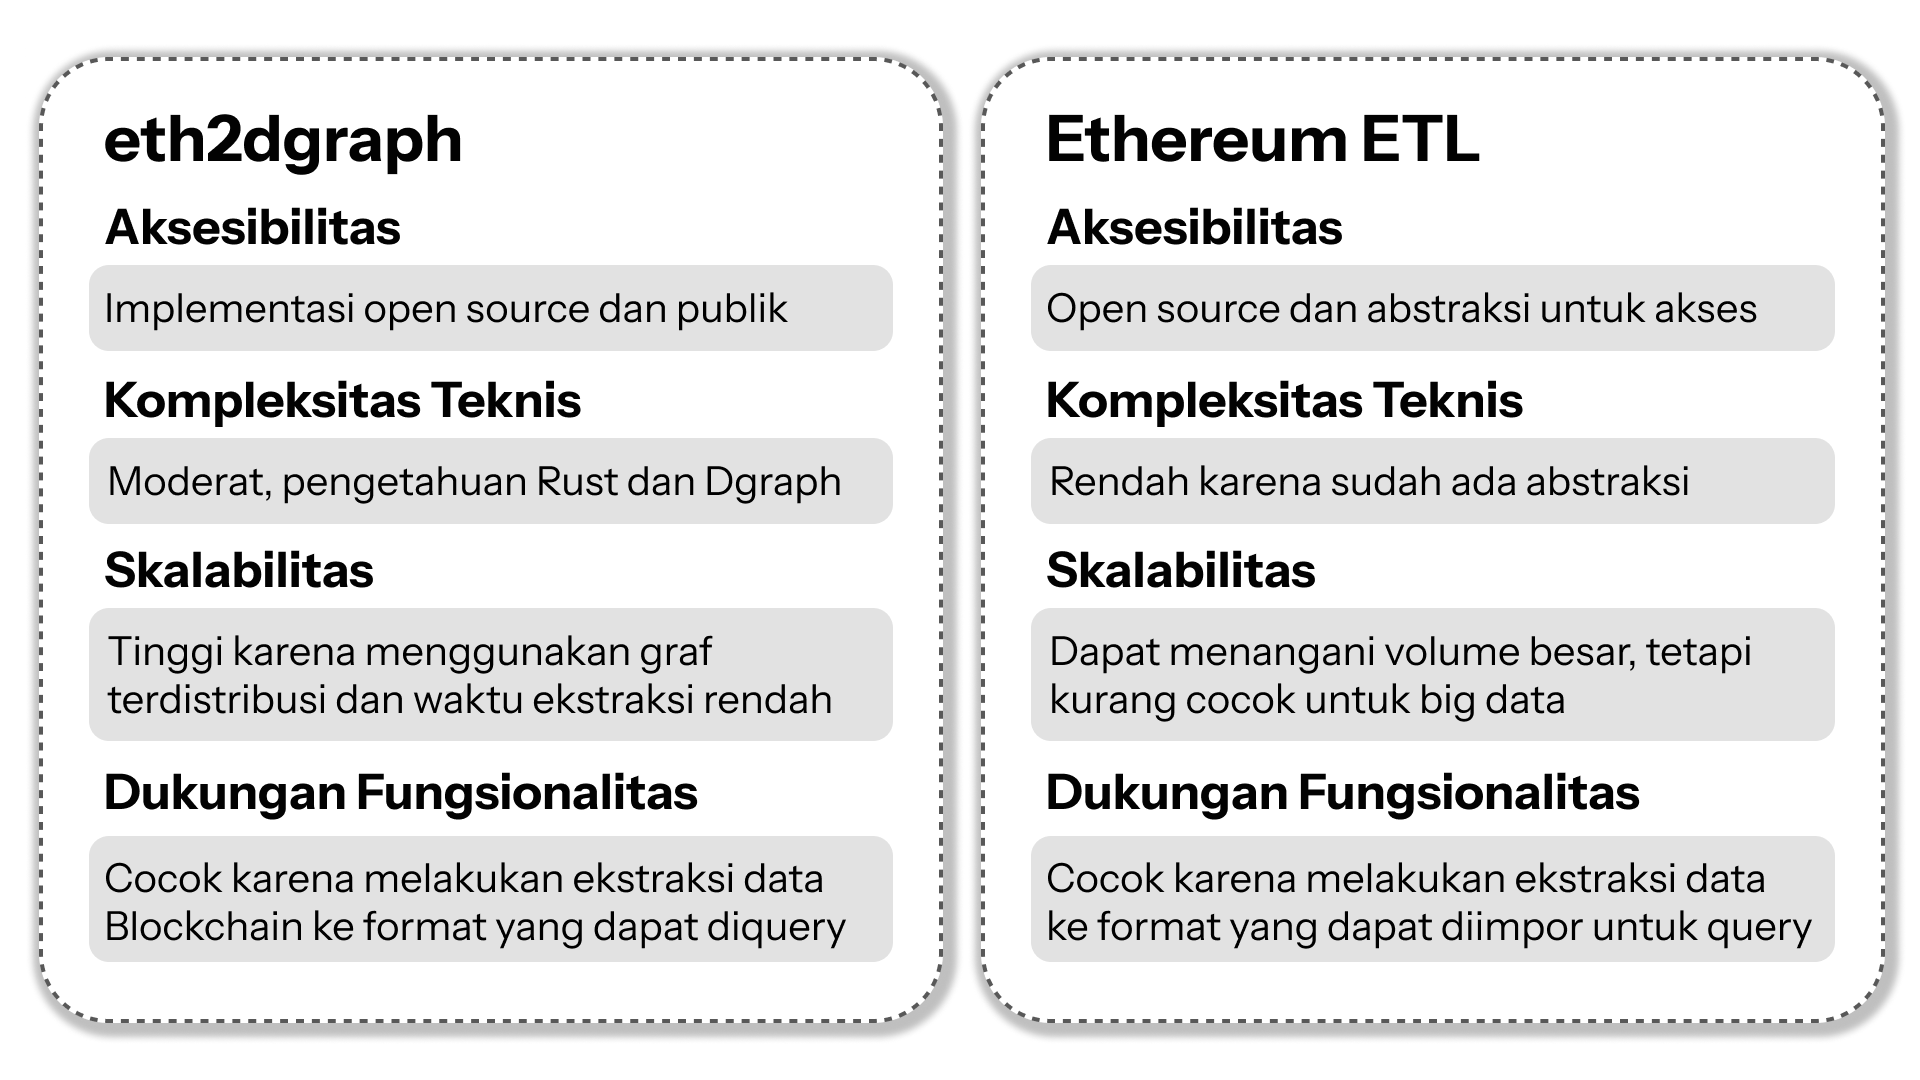
\includegraphics[width=0.9\textwidth]{resources/chapter-3/ekstraksi-1.png}
	\caption{Perbandingan alternatif ekstraksi data Smart Contracts dari Blockchain Ethereum}
	\label{image:perbandingan-ekstraksi-1}
\end{figure}

\begin{figure}[ht]
	\centering
	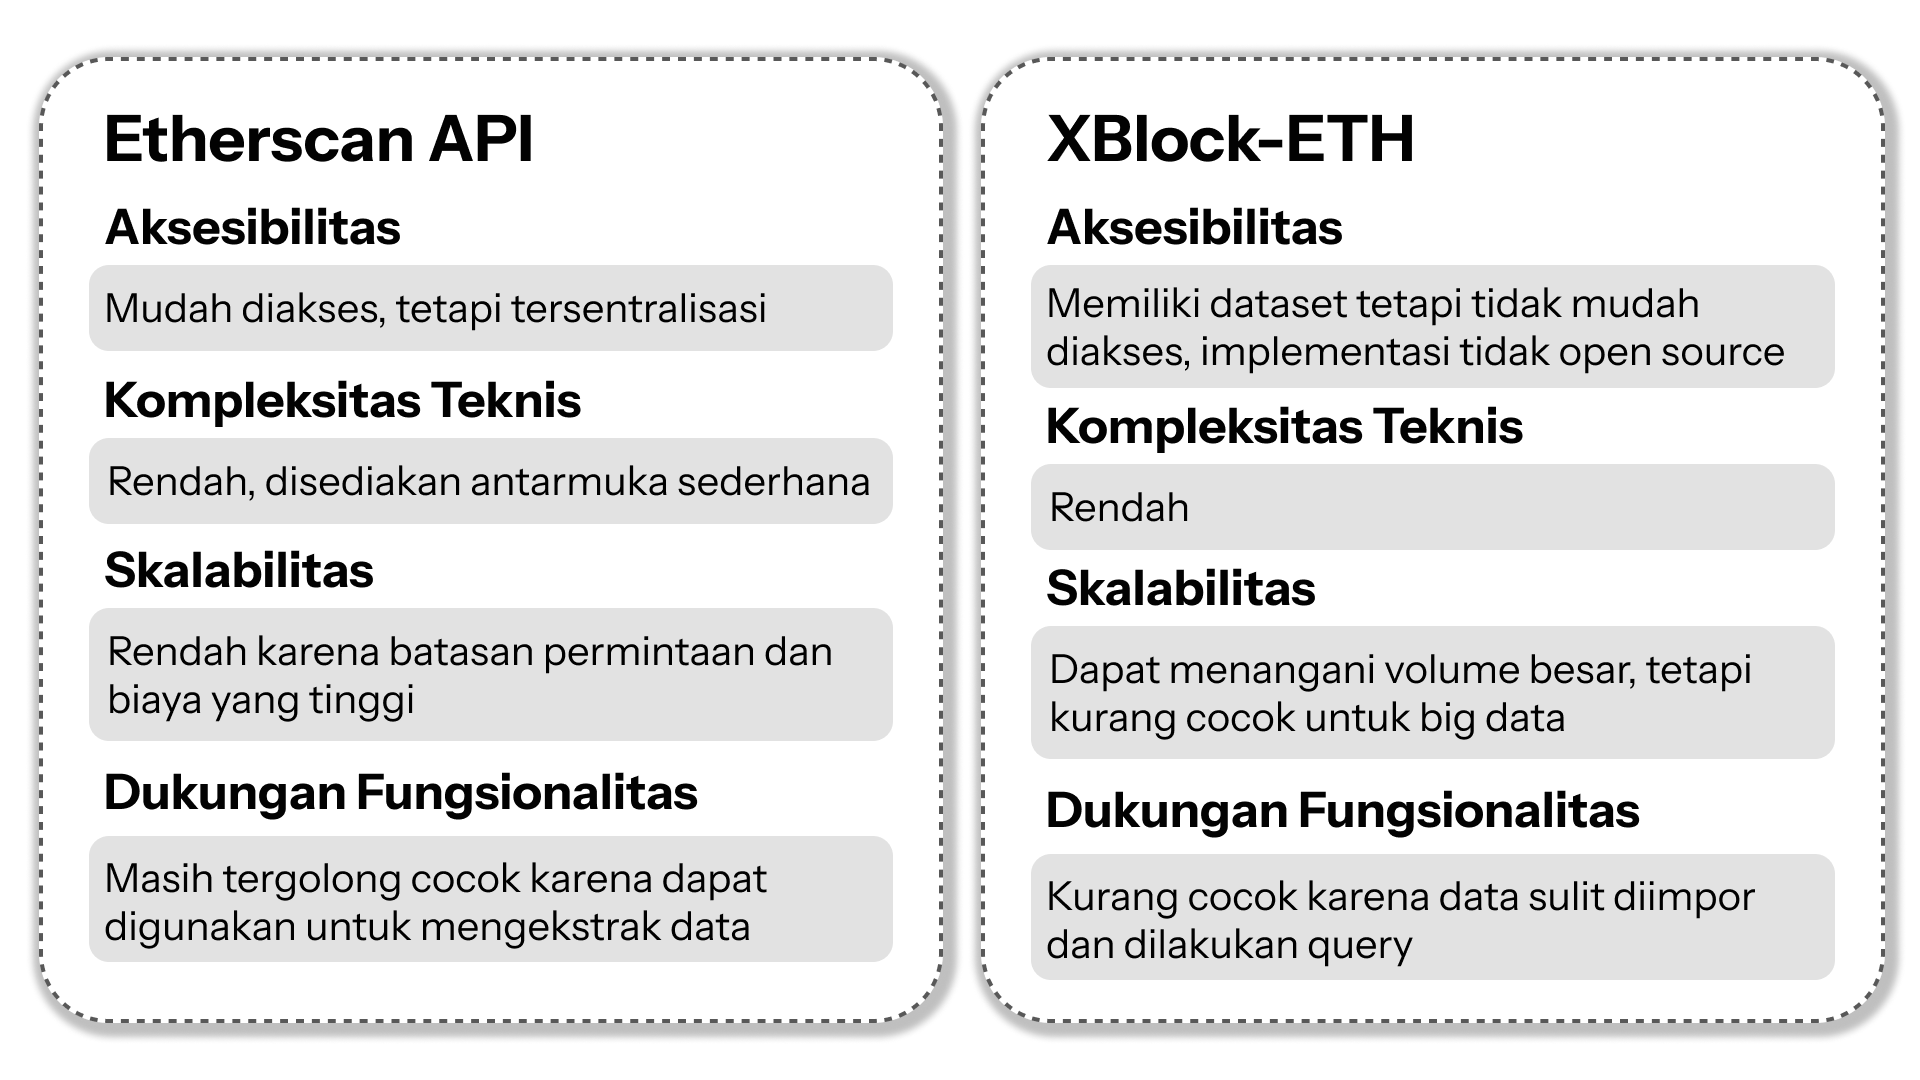
\includegraphics[width=0.9\textwidth]{resources/chapter-3/ekstraksi-2.png}
	\caption{Perbandingan alternatif ekstraksi data Smart Contracts dari Blockchain Ethereum}
	\label{image:perbandingan-ekstraksi-2}
\end{figure}

\begin{figure}[ht]
	\centering
	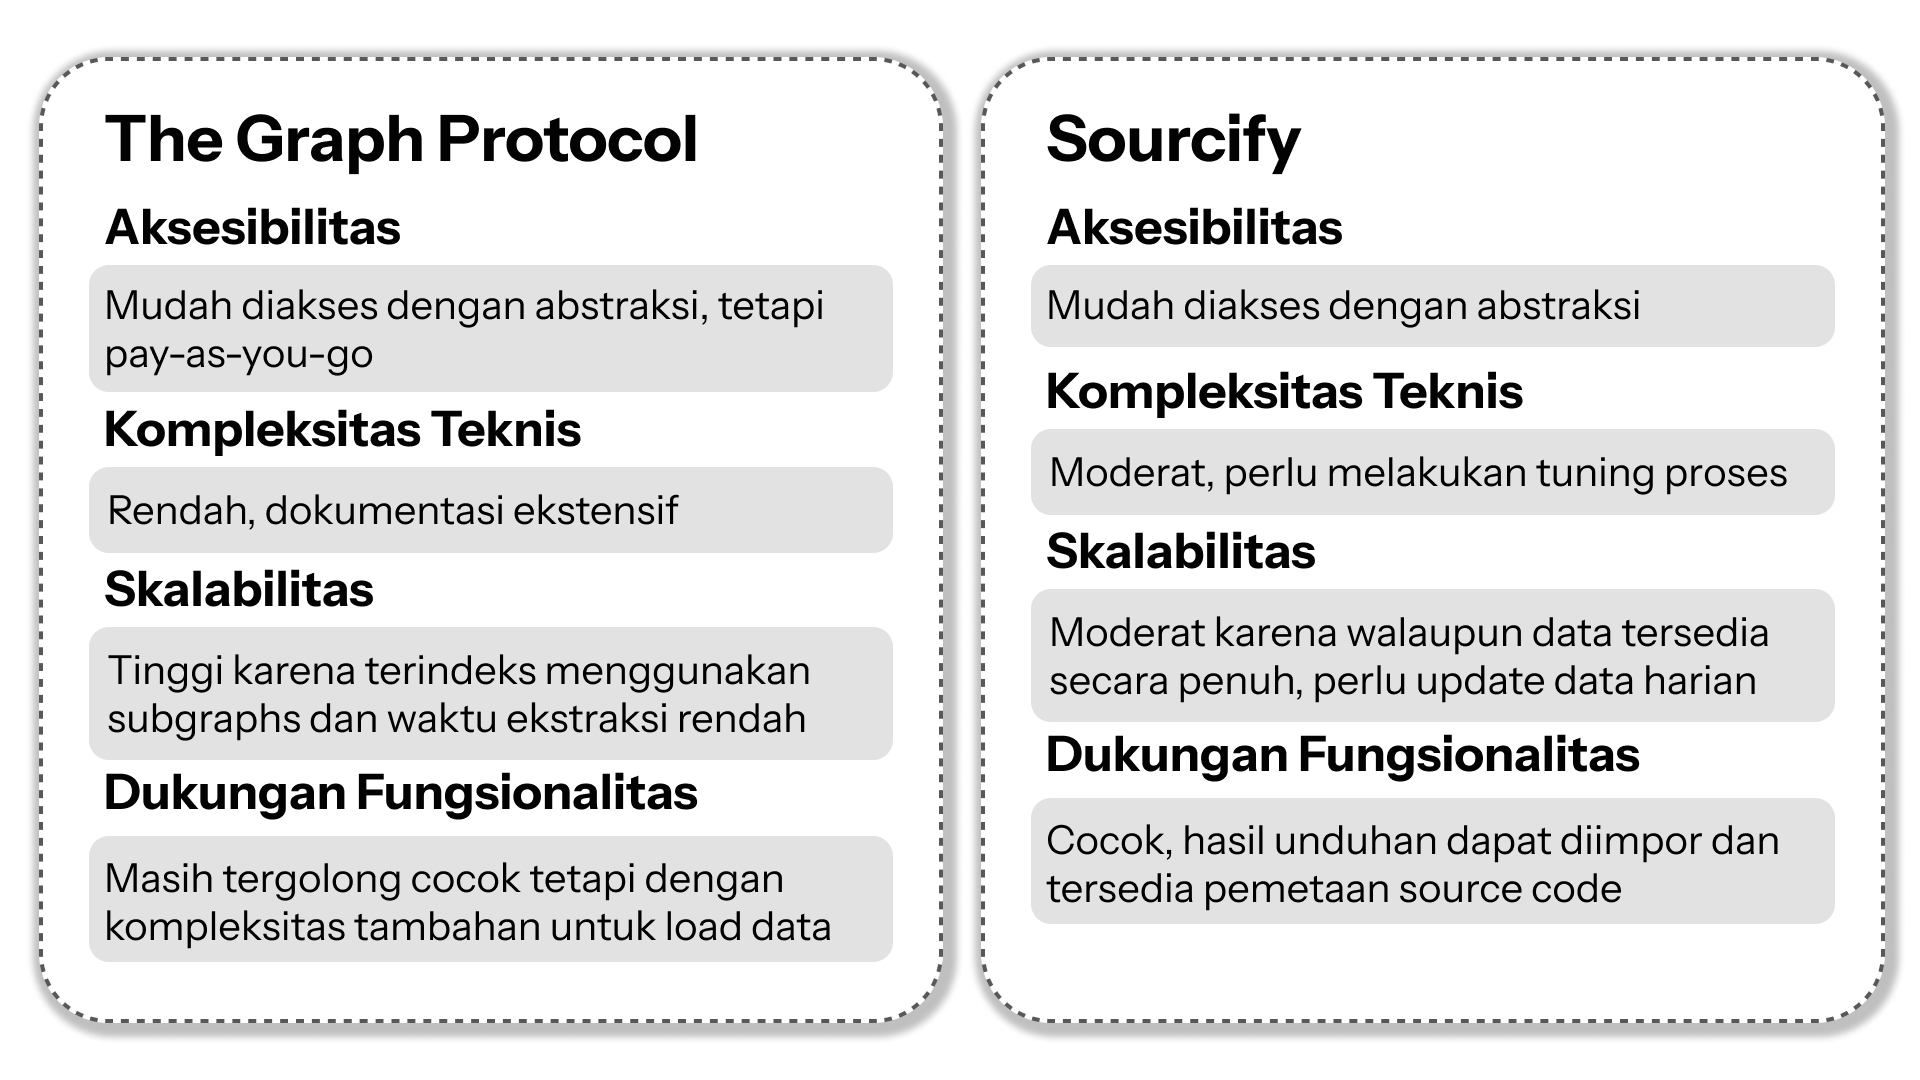
\includegraphics[width=0.9\textwidth]{resources/chapter-3/ekstraksi-3.png}
	\caption{Perbandingan alternatif ekstraksi data Smart Contracts dari Blockchain Ethereum}
	\label{image:perbandingan-ekstraksi-3}
\end{figure}

Kebutuhan pertama yang harus dipenuhi adalah ekstraksi data Smart Contracts dari Blockchain Ethereum. Proses ini mencakup pengambilan data terkait Smart Contracts, seperti ABI, bytecode, metadata, dan Verified \textit{source code}. Data ini akan digunakan untuk membangun basis data yang dapat di-query dan dianalisis lebih lanjut.

Dukungan fungsional yang diperlukan tidak hanya mencakup ekstraksi data, tetapi juga kemampuan memperoleh source code yang terverifikasi dan memetakan source code tersebut dengan deployment untuk analisis tanpa dekompilasi. Prioritas fungsionalnya adalah menghasilkan data dalam format siap pakai, memperoleh source code, dan mengaitkannya dengan deployment.

Gambar \ref{image:perbandingan-ekstraksi-1}, \ref{image:perbandingan-ekstraksi-2}, dan \ref{image:perbandingan-ekstraksi-3} menunjukkan rangkuman perbandingan berbagai alternatif ekstraksi data Smart Contracts dari Blockchain Ethereum. Secara rinci, berikut adalah analisis dari masing-masing alternatif:

\begin{enumerate}
	\item \textbf{eth2dgraph} \parencite{aimar2023extraction}: Riset ini unggul dalam mengekstrak ABI, bytecode, dan metadata yang dikonversi menjadi format graf. Implementasinya yang \textit{open source} menggunakan Rust untuk kinerja tinggi dan Dgraph untuk skalabilitas, sehingga memungkinkan query pada hubungan antar Smart Contracts di Ethereum. Pendekatan ini memerlukan \textit{node} Ethereum dan dasar pengetahuan mengenai Rust dan Dgraph. Selain ekstraksi cepat, eth2dgraph efektif dalam mengaitkan Smart Contracts Deployment dengan Verified \textit{source code} serta dapat diperluas untuk menambahkan aspek semantik.

	\item \textbf{Ethereum ETL} \parencite{ethereum_etl}: Ethereum ETL dikenal karena kemudahan penggunaan dan dokumentasinya yang lengkap, serta dukungan untuk data transaksi, blok, dan Smart Contracts. Meskipun demikian, ia tidak mendukung ekstraksi ABI, membutuhkan waktu lebih lama, dan memerlukan beberapa operasi tambahan untuk memperoleh data Smart Contracts. Hasil ekstraksinya cocok untuk basis data relasional, namun kurang ideal untuk sistem big data karena format data yang dihasilkan.

	\item \textbf{Etherscan API} \parencite{etherscan2024}: Dengan Etherscan API, pengguna dapat langsung mengekstrak data Smart Contracts beserta Verified \textit{source code} dari sumber yang terpercaya. Antarmukanya yang sederhana memudahkan akses, namun seluruh data bergantung pada Etherscan yang tersentralisasi. Batasan jumlah permintaan serta biaya penggunaan juga perlu diperhitungkan, terutama untuk ekstraksi data skala besar.

	\item \textbf{XBlock-ETH} \parencite{zheng2020xblock}: XBlock-ETH memungkinkan ekstraksi data tanpa memanfaatkan \textit{node} Ethereum, namun hasilnya disimpan dalam bentuk CSV yang memerlukan parsing tambahan dan tidak mendukung query atau indexing secara efisien. Selain itu, karena kode ekstraksinya tidak \textit{open source}, replikasi proses menjadi sulit meskipun pendekatannya cukup sederhana untuk digunakan.

	\item \textbf{The Graph Protocol} \parencite{TheGraphDocs}: The Graph menawarkan kemudahan penggunaan dengan query cepat dan infrastruktur yang terintegrasi dengan baik. Namun, model pembayaran \textit{pay-as-you-go} dapat membuat biaya ekstraksi data meningkat. Data JSON yang dihasilkan memerlukan konversi ulang ke format lain, meski flexibelnya memudahkan pengembangan lebih lanjut.

	\item \textbf{Sourcify} \parencite{sourcify_website}: Sourcify menyediakan antarmuka yang mudah untuk mengunduh dan memetakan hubungan antara \textit{source code} dan Deployment. Meskipun sudah tersedia abstraksi, ia tidak mendukung ekstraksi data kompleks seperti ABI dan bytecode. Proses pengunduhan berkala untuk memperbarui data masih perlu dioptimalkan agar lebih efisien, meskipun penggunaannya tergolong moderat.
\end{enumerate}


\subsubsection{Pemodelan, Penyimpanan, dan \textit{Indexing} Data Smart Contracts}

% jadi bahas alternatif dulu, misal yang terpilih eth2dgraph
% lalu bahas schema yang dipakainya gimana, yang base nya apa aja secara singkat, dan yang mau ditambahinnya apa, berdasarkan apa
% Jadiin dua subheading

\subsubsection{Klasifikasi Fungsional dan Semantik Smart Contracts}

\begin{figure}[ht]
	\centering
	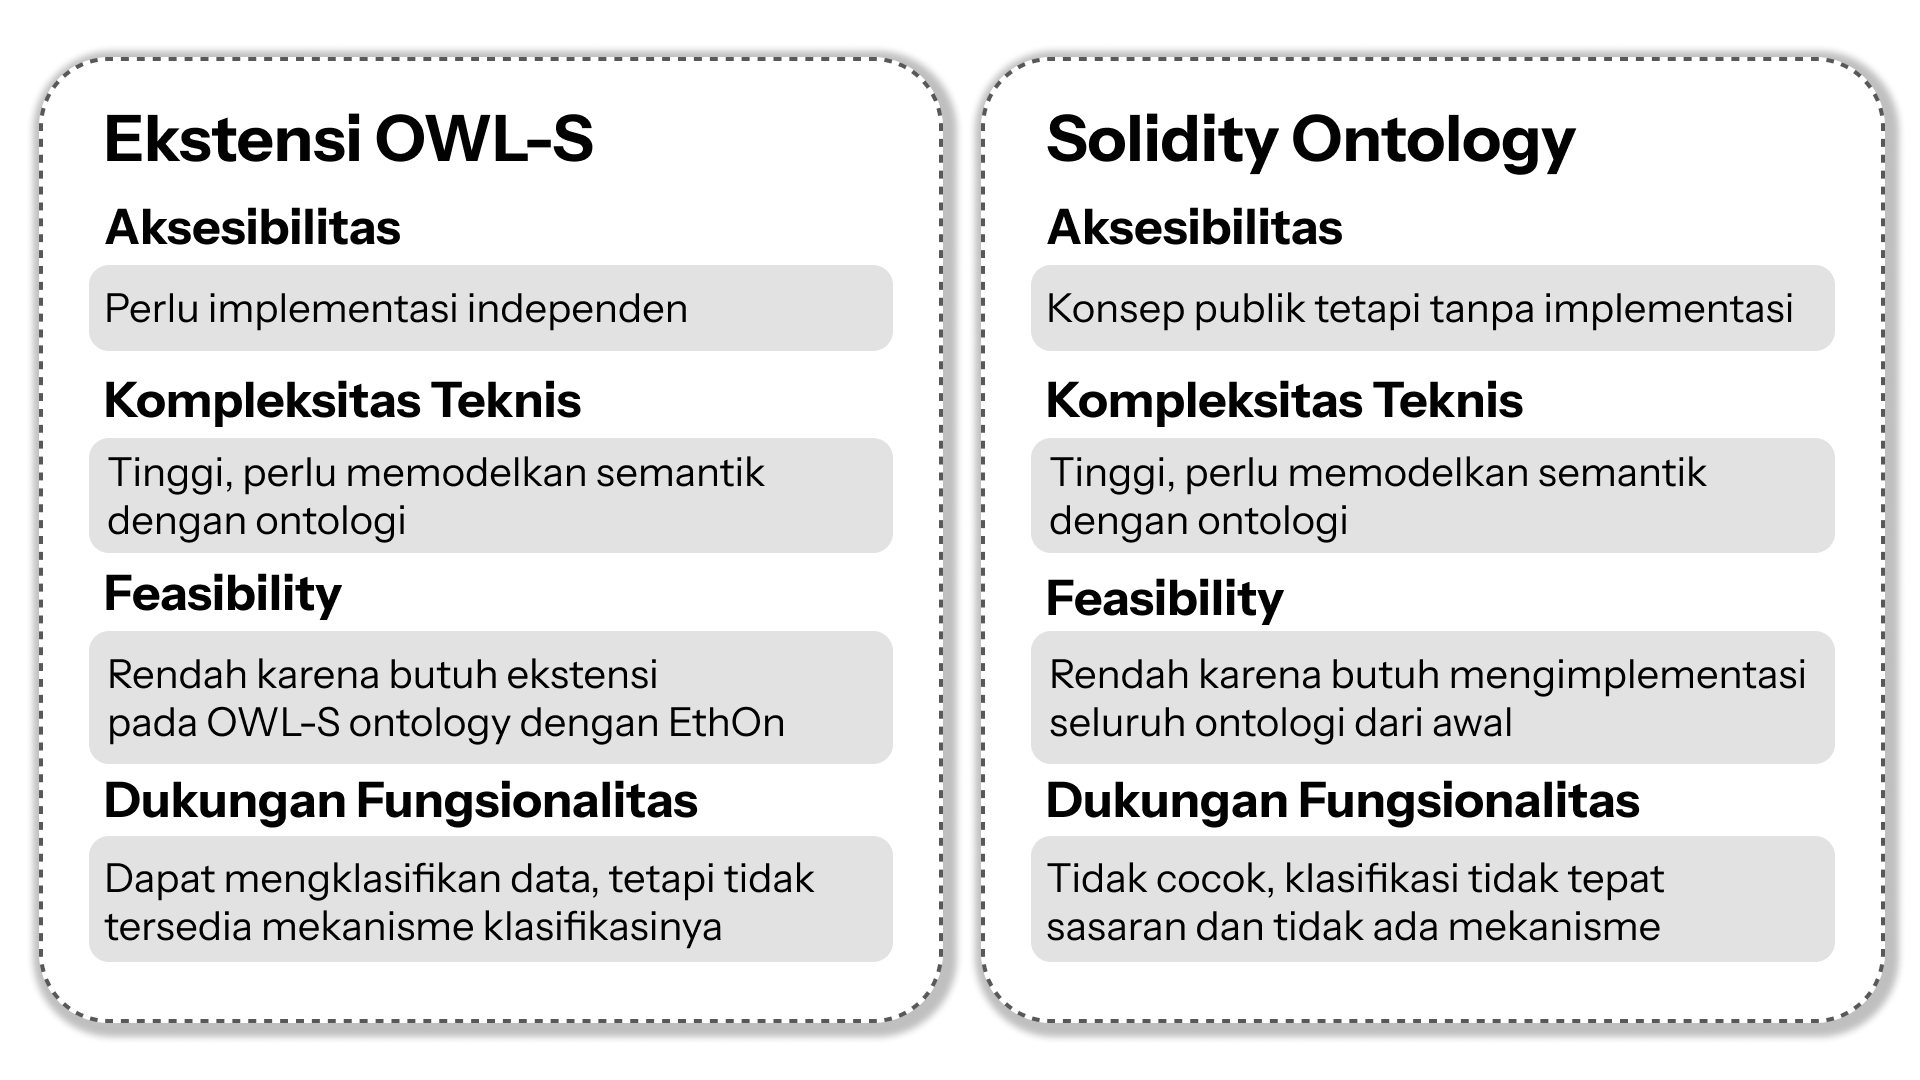
\includegraphics[width=0.9\textwidth]{resources/chapter-3/klasifikasi - 1.png}
	\caption{Perbandingan alternatif klasifikasi fungsional dan semantik Smart Contracts}
	\label{image:klasifikasi-1}
\end{figure}

\begin{figure}[ht]
	\centering
	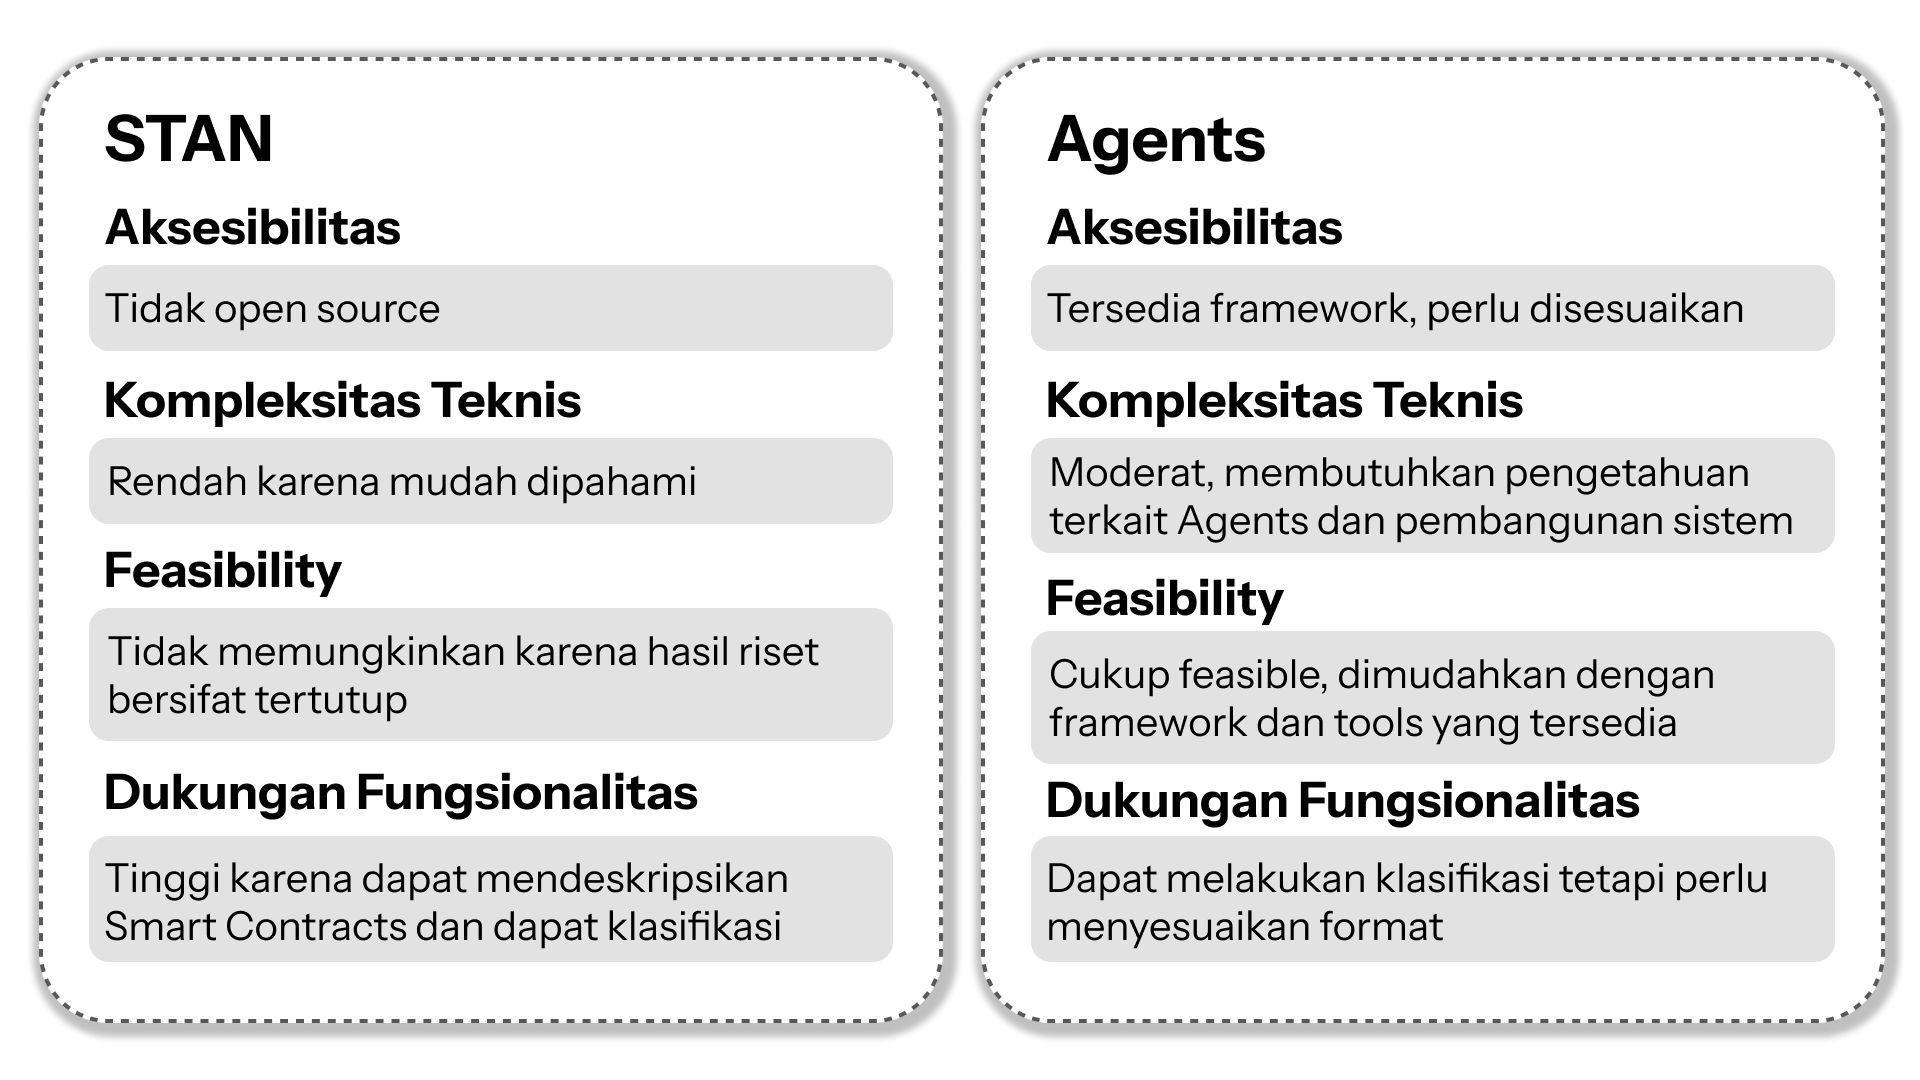
\includegraphics[width=0.9\textwidth]{resources/chapter-3/klasifikasi - 2.png}
	\caption{Perbandingan alternatif klasifikasi fungsional dan semantik Smart Contracts}
	\label{image:klasifikasi-2}
\end{figure}

\begin{figure}[ht]
	\centering
	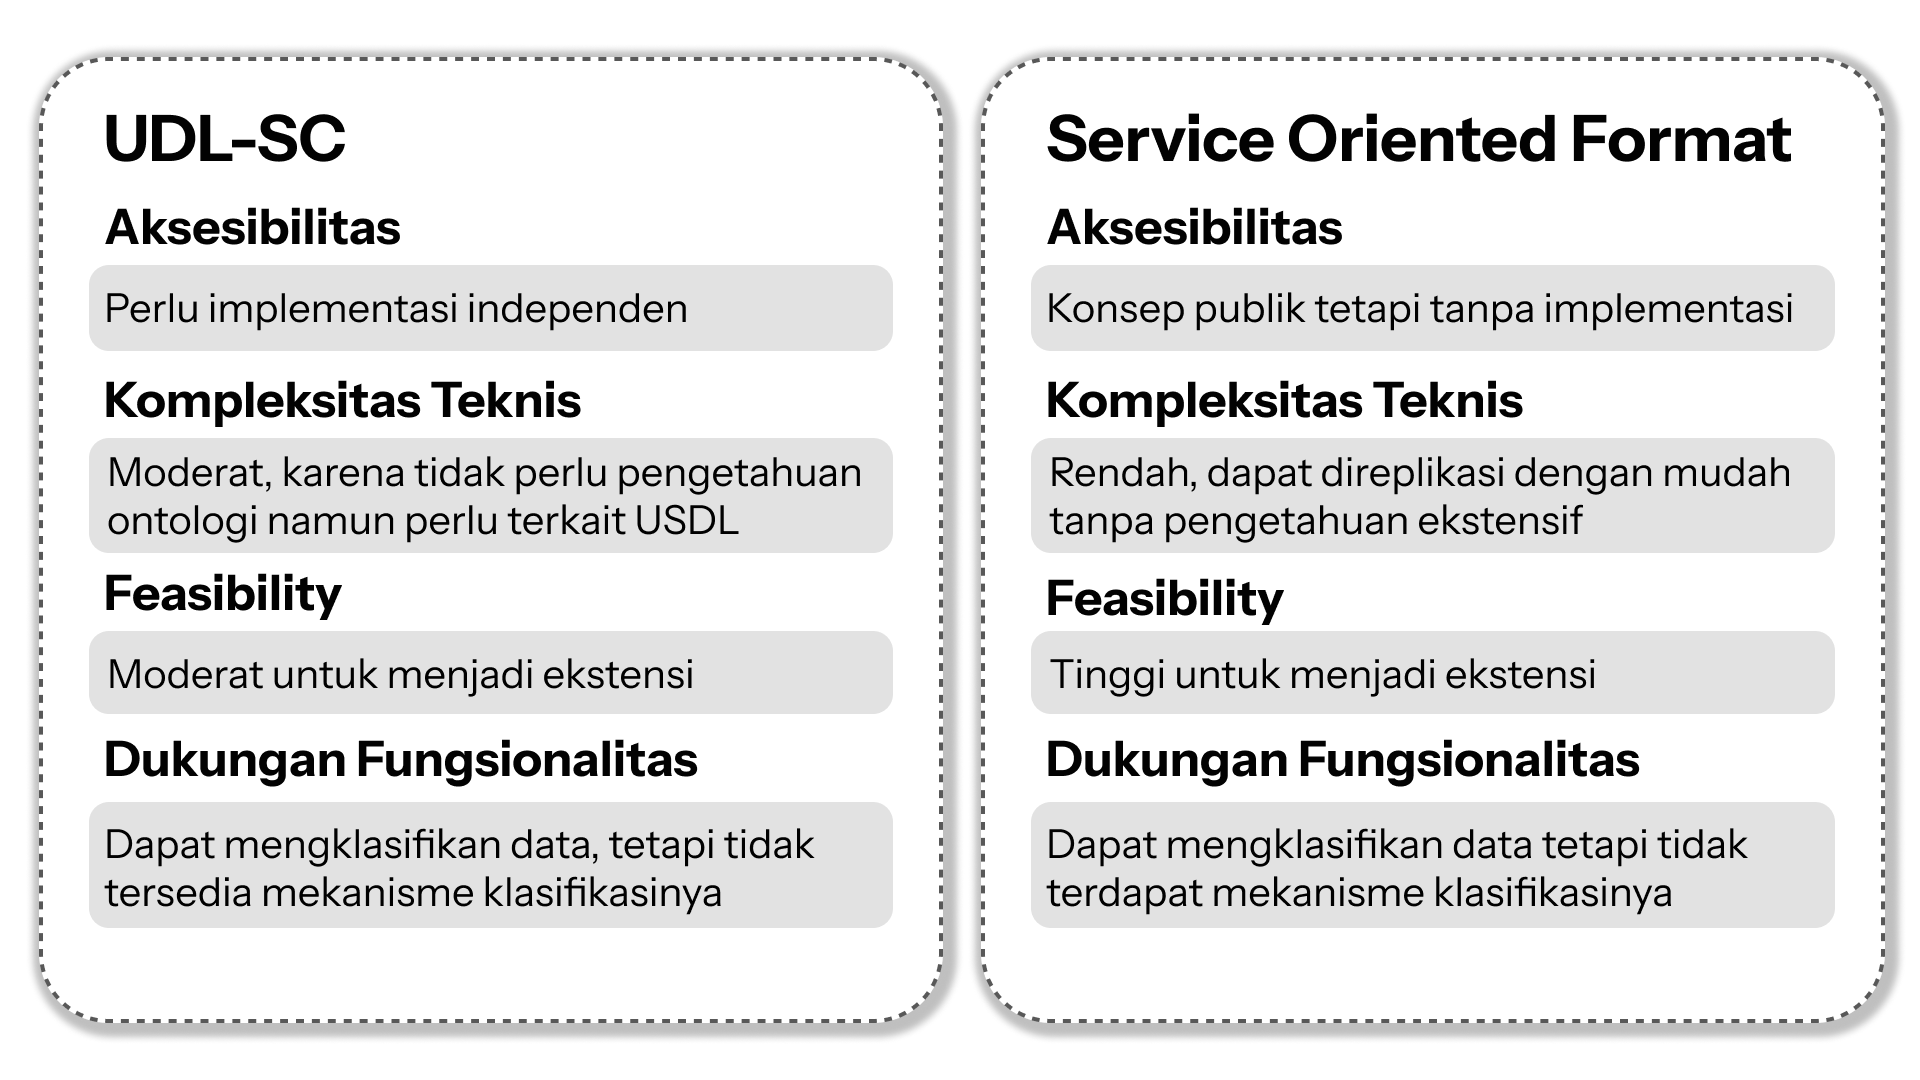
\includegraphics[width=0.9\textwidth]{resources/chapter-3/klasifikasi - 3.png}
	\caption{Perbandingan alternatif klasifikasi fungsional dan semantik Smart Contracts}
	\label{image:klasifikasi-3}
\end{figure}

\begin{figure}[ht]
	\centering
	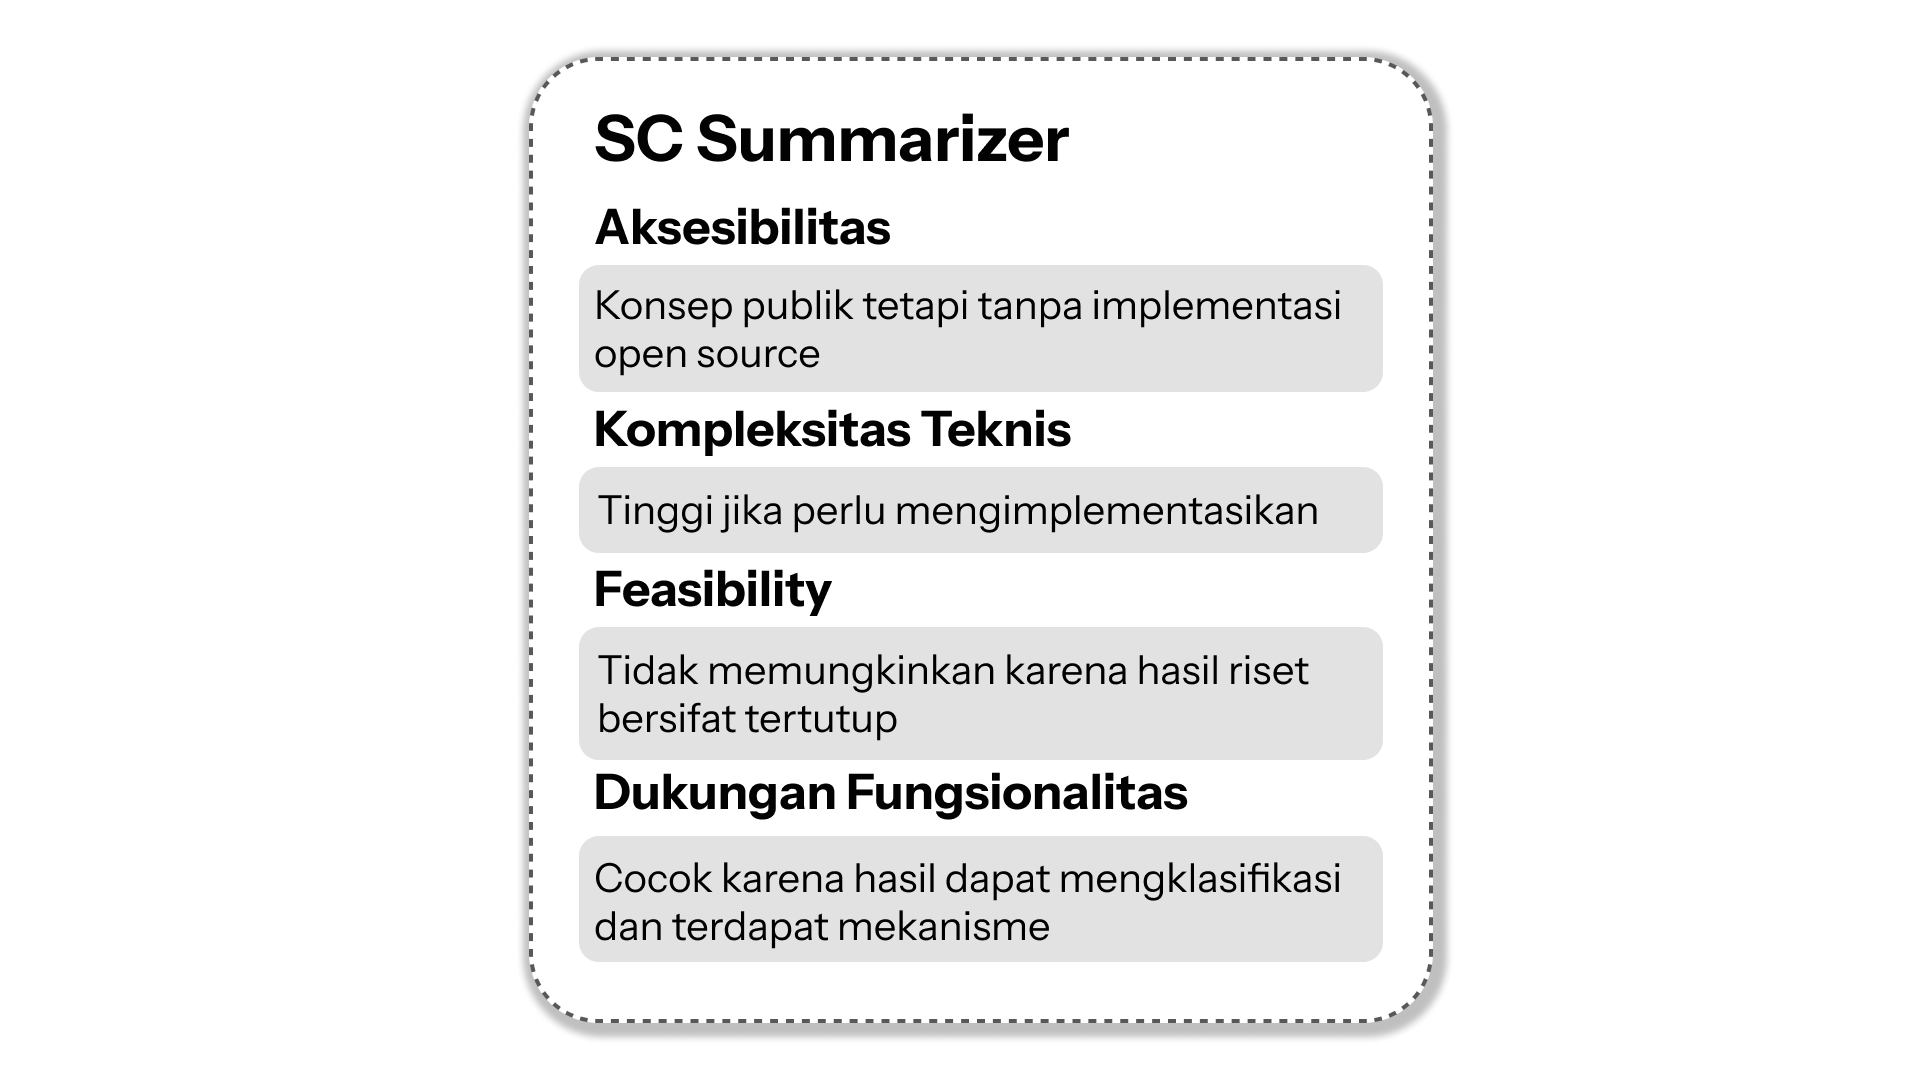
\includegraphics[width=0.9\textwidth]{resources/chapter-3/klasifikasi - 4.png}
	\caption{Perbandingan alternatif klasifikasi fungsional dan semantik Smart Contracts}
	\label{image:klasifikasi-4}
\end{figure}

Data yang sudah dimodelkan dan disimpan ke dalam sistem perlu dilakukan klasifikasi untuk memudahkan pencarian Smart Contracts berdasarkan fungsionalitas dan semantik. Terdapat berbagai alternatif untuk melakukan klasifikasi fungsional dan semantik Smart Contracts dengan berbagai pendekatan, baik dengan pemodelan ontologi, deskripsi fungsional, maupun format lainnya. Dukungan fungsional yang baik untuk klasifikasi adalah riset yang dapat melakukan klasifikasi pada data Smart Contracts dengan baik dan memberikan deskripsi atau hasil klasifikasi yang baik. Pada bagian ini, aspek skalabilitas digantikan dengan aspek \textit{feasibility}.

Gambar \ref{image:klasifikasi-1}, \ref{image:klasifikasi-2}, \ref{image:klasifikasi-3}, dan \ref{image:klasifikasi-4} menunjukkan rangkuman perbandingan berbagai alternatif klasifikasi fungsional dan semantik Smart Contracts. Secara rinci, berikut adalah analisis dari masing-masing alternatif:

\begin{enumerate}
	\item \textbf{Semantic Smart Contracts for Blockchain-based Services in the Internet of Things} \parencite{baqa2019semantic} (Bagian \ref{subsec:semantic-smart-contract-iot}): Riset ini menggunakan ekstensi pada OWL-S Service Ontology untuk melakukan klasifikasi Smart Contracts berdasarkan semantik dan fungsionalitas. Keunggulannya adalah penggunaan ontologi yang dapat di-\textit{extend} untuk menambahkan terminologi yang \textit{domain specific}. Secara aksesibilitas, riset ini bersifat \textit{public}, namun tidak memiliki implementasi \textit{open source}. Selain itu, riset ini terbatas pada \textit{scope} Internet-of-Things. Secara kompleksitas, riset ini tergolong tinggi karena memerlukan pemahaman yang mendalam tentang ontologi dan pemodelan semantik. Dalam hal dukungan fungsional, riset ini dapat memberikan deskripsi yang baik, tetapi tidak terdapat mekanisme untuk mengklasifikasikan data dengan baik.

	\item \textbf{Ontological Modeling of Smart Contracts in Solidity} \parencite{cano2021toward} (Bagian \ref{subsec:solidity-ontology}): Riset ini menerapkan ontologi pada bahasa pemrograman Solidity. Ontologi ini digunakan untuk mendeskripsikan elemen-elemen dalam Smart Contracts, seperti fungsi, variabel, dan struktur data. Secara aksesibilitas, riset ini bersifat publik, dengan ontologi yang dihasilkan dapat diterapkan. Namun, implementasi ontologi pada riset ini terbatas pada sintaks dan semantik dari kode bahasa pemrograman Solidity sendiri dibandingkan Smart Contracts secara keseluruhan. Secara kompleksitas, riset ini tergolong tinggi karena memerlukan pemahaman yang mendalam tentang ontologi dan pemodelan semantik, dan memerlukan proses klasifikasi yang ekstensif untuk memetakan data dengan ontologi yang dihasilkan. Dalam hal dukungan fungsional, riset ini tidak sesuai dengan kebutuhan sistem, yaitu memodelkan fungsionalitas dari Smart Contract, bukan aspek sintaks bahasa pemrograman Soliditynya, dan tidak terdapat mekanisme untuk mengklasifikasikan data dengan baik.

	\item \textbf{STAN} \parencite{stan} (Bagian \ref{subsec:stan}): STAN adalah sebuah sistem untuk memberikan deskripsi terhadap bytecodes dari Smart Contracts. Secara aksesibilitas, STAN tidak bersifat \textit{open source}, sehingga tidak tersedia implementasinya untuk melakukan replikasi. Secara kompleksitas, STAN tergolong rendah karena abstraksi yang sudah diberikan untuk menghasilkan deskripsi. Riset STAN ini juga belum menginkorporasikan teknologi seperti Artificial Intelligence (AI) untuk melakukan klasifikasi. Dalam hal dukungan fungsional, STAN dapat membantu mengklasifikasikan Smart Contracts berdasarkan deskripsi yang dihasilkan.

	% \item \textbf{Agents} (Bagian \ref{sec:agents}): Alternatif untuk melakukan klasifikasi Smart Contracts adalah menggunakan AI Agents yang dapat melakukan dekomposisi tasks yang kompleks menjadi sub-tasks yang lebih sederhana. Dengan menggunakan AI Agents, klasifikasi Smart Contracts dapat dilakukan dengan lebih menyeluruh dan efisien karena dapat memperhitungkan berbagai aspek yang ada pada Smart Contracts. Secara aksesibilitas, sudah banyak \textit{framework} dan \textit{tools} yang tersedia untuk membangun sebuah sistem berbasis AI Agents (Agentic AI). Namun, perlu dilakukan pembangunan secara independen karena tidak ada sistem yang secara langsung memberikan fungsionalitas yang sesuai. Secara kompleksitas, penggunaan AI Agents tergolong moderat karena memerlukan pengetahuan terkait AI dan membuat sistem berbasis AI Agents. Secara \textit{feasibility}, pembangunan sistem berbasis agents cukup \textit{feasible} dengan penggunaan \textit{framework} dan \textit{tools} yang baik. Dukungan fungsional yang diberikan oleh sistem dengan AI Agents tergolong baik karena dapat disesuaikan dan melakukan pekerjaan kompleks secara otonom, tetapi perlu menggunakan format yang disesuaikan untuk mendeskripsikan data.
	      % menggunakan agents yang dimasukkin source code, dengan break down step by step

	\item \textbf{LLM Classification} (Bagian \ref{sec:llms}): Penggunaan LLM untuk melakukan klasifikasi Smart Contracts dengan menghasilkan deskripsi dan mengklasifikasikan berdasarkan deskripsi yang dihasilkan. Dengan memanfaatkan kemampuan LLM dalam memahami konteks dan semantik, diharapkan klasifikasi dapat dilakukan dengan lebih akurat dan efisien. Secara aksesibilitas, LLMs seperti GPT-4 dan Llama-3 sudah tersedia untuk digunakan, baik melalui API maupun model yang dapat diunduh. Secara kompleksitas, penggunaan LLMs tergolong rendah karena hanya memerlukan pengetahuan dasar tentang pemrograman dan penggunaan API. Secara \textit{feasibility}, sistem ini \textit{feasible} untuk diimplementasikan dengan infrastruktur yang ada. Dalam hal dukungan fungsional, LLMs dapat memberikan deskripsi yang baik dan melakukan klasifikasi Smart Contracts dengan baik, tetapi perlu diperhatikan bahwa LLMs tidak selalu memberikan hasil yang konsisten.

	\item \textbf{Uniform Description Language for Smart Contracts} \parencite{udlsc} (Bagian \ref{subsec:uniform-description-language}): Riset ini mengusulkan sebuah bahasa deskripsi ekstensi dari USDL untuk Smart Contracts. Secara aksesibilitas, hasil dari riset ini bersifat \textit{public}, namun perlu melakukan replikasi untuk mendapatkan hasil yang didapatkan dari riset. Secara kompleksitas, riset ini tergolong moderat karena walaupun tidak memerlukan pengetahuan yang mendalam terkait ontologi, perlu memahami terkait USDL dan implementasi ekstensi dari USDL. Secara skalabilitas, riset ini tergolong baik karena dapat digunakan sebagai ekstensi data tanpa masalah. Dalam hal dukungan fungsional, riset ini kurang baik karena tidak terdapat mekanisme untuk mengklasifikasikan data dengan baik, tetapi dapat digunakan untuk mendeskripsikan data Smart Contracts dengan baik.

	\item \textbf{Service Oriented Format Descriptor} \parencite{guida2019supporting} (Bagian \ref{subsec:supporting-reuse-smart-contracts}): Riset ini mengusulkan sebuah format deskripsi untuk Smart Contracts dengan pendekatan Service. Riset ini juga mengusulkan sebuah Service Registry dan Contract Editor berbasis visual yang mengkomplemen format deskripsi yang diusulkan. Format deskripsi ini dapat digunakan dan digabungkan dengan sistem lain, sedangkan Service Registry dan Contract Editor kurang fleksibel untuk diintegrasikan dengan sistem lain. Secara aksesibilitas, hasil dari riset ini bersifat \textit{public} dan \textit{open source}, sehingga dapat digunakan untuk melakukan replikasi. Secara kompleksitas, format yang dihasilkan oleh riset ini tergolong rendah karena tidak memerlukan pengetahuan yang mendalam dan dapat langsung dijadikan ekstensi ke format lain. Dalam hal dukungan fungsional, riset ini dapat mengakomodasi deskripsi Smart Contracts dengan baik, tetapi tidak ada mekanisme untuk melakukan klasifikasi data dengan baik.

	\item \textbf{Smart Contract Summarizer} \parencite{zhang2021smart} (Bagian \ref{subsec:smart-contract-solidity-summary}): Riset ini mengusulkan sebuah sistem untuk menghasilkan ringkasan dan anotasi dari Smart Contracts, terutama dalam bahasa Solidity. Sistem ini menggunakan teknik NLG (Natural Language Generation) dengan pendekatan berbasis \textit{transformer} untuk menghasilkan ringkasan yang lebih baik dibandingkan dengan metode berbasis template sebelumnya. Secara aksesibilitas, konsep dari riset ini bersifat \textit{public}, namun tidak memiliki implementasi \textit{open source}. Secara kompleksitas, jika perlu mengimplementasikan dari awal, riset ini tergolong tinggi karena memerlukan pengetahuan yang mendalam terkait NLP dan pemodelan semantik. Secara skalabilitas, sistem ini tidak diketahui untuk kinerja menangani data yang banyak. Dalam hal dukungan fungsional, riset ini dapat membantu mengklasifikasikan Smart Contracts berdasarkan ringkasan yang dihasilkan dengan mekanisme yang digunakan.

\end{enumerate}


\subsubsection{Pencarian dan Rekomendasi Smart Contracts}

% ini LLM, terus pake langchain?? (iya si harusnya (recheck obsidian pls))

\subsubsection{Interaksi Pengguna dengan Sistem}


\subsubsection{Kesimpulan Pemilihan Alternatif}

\begin{figure}[ht]
	\centering
	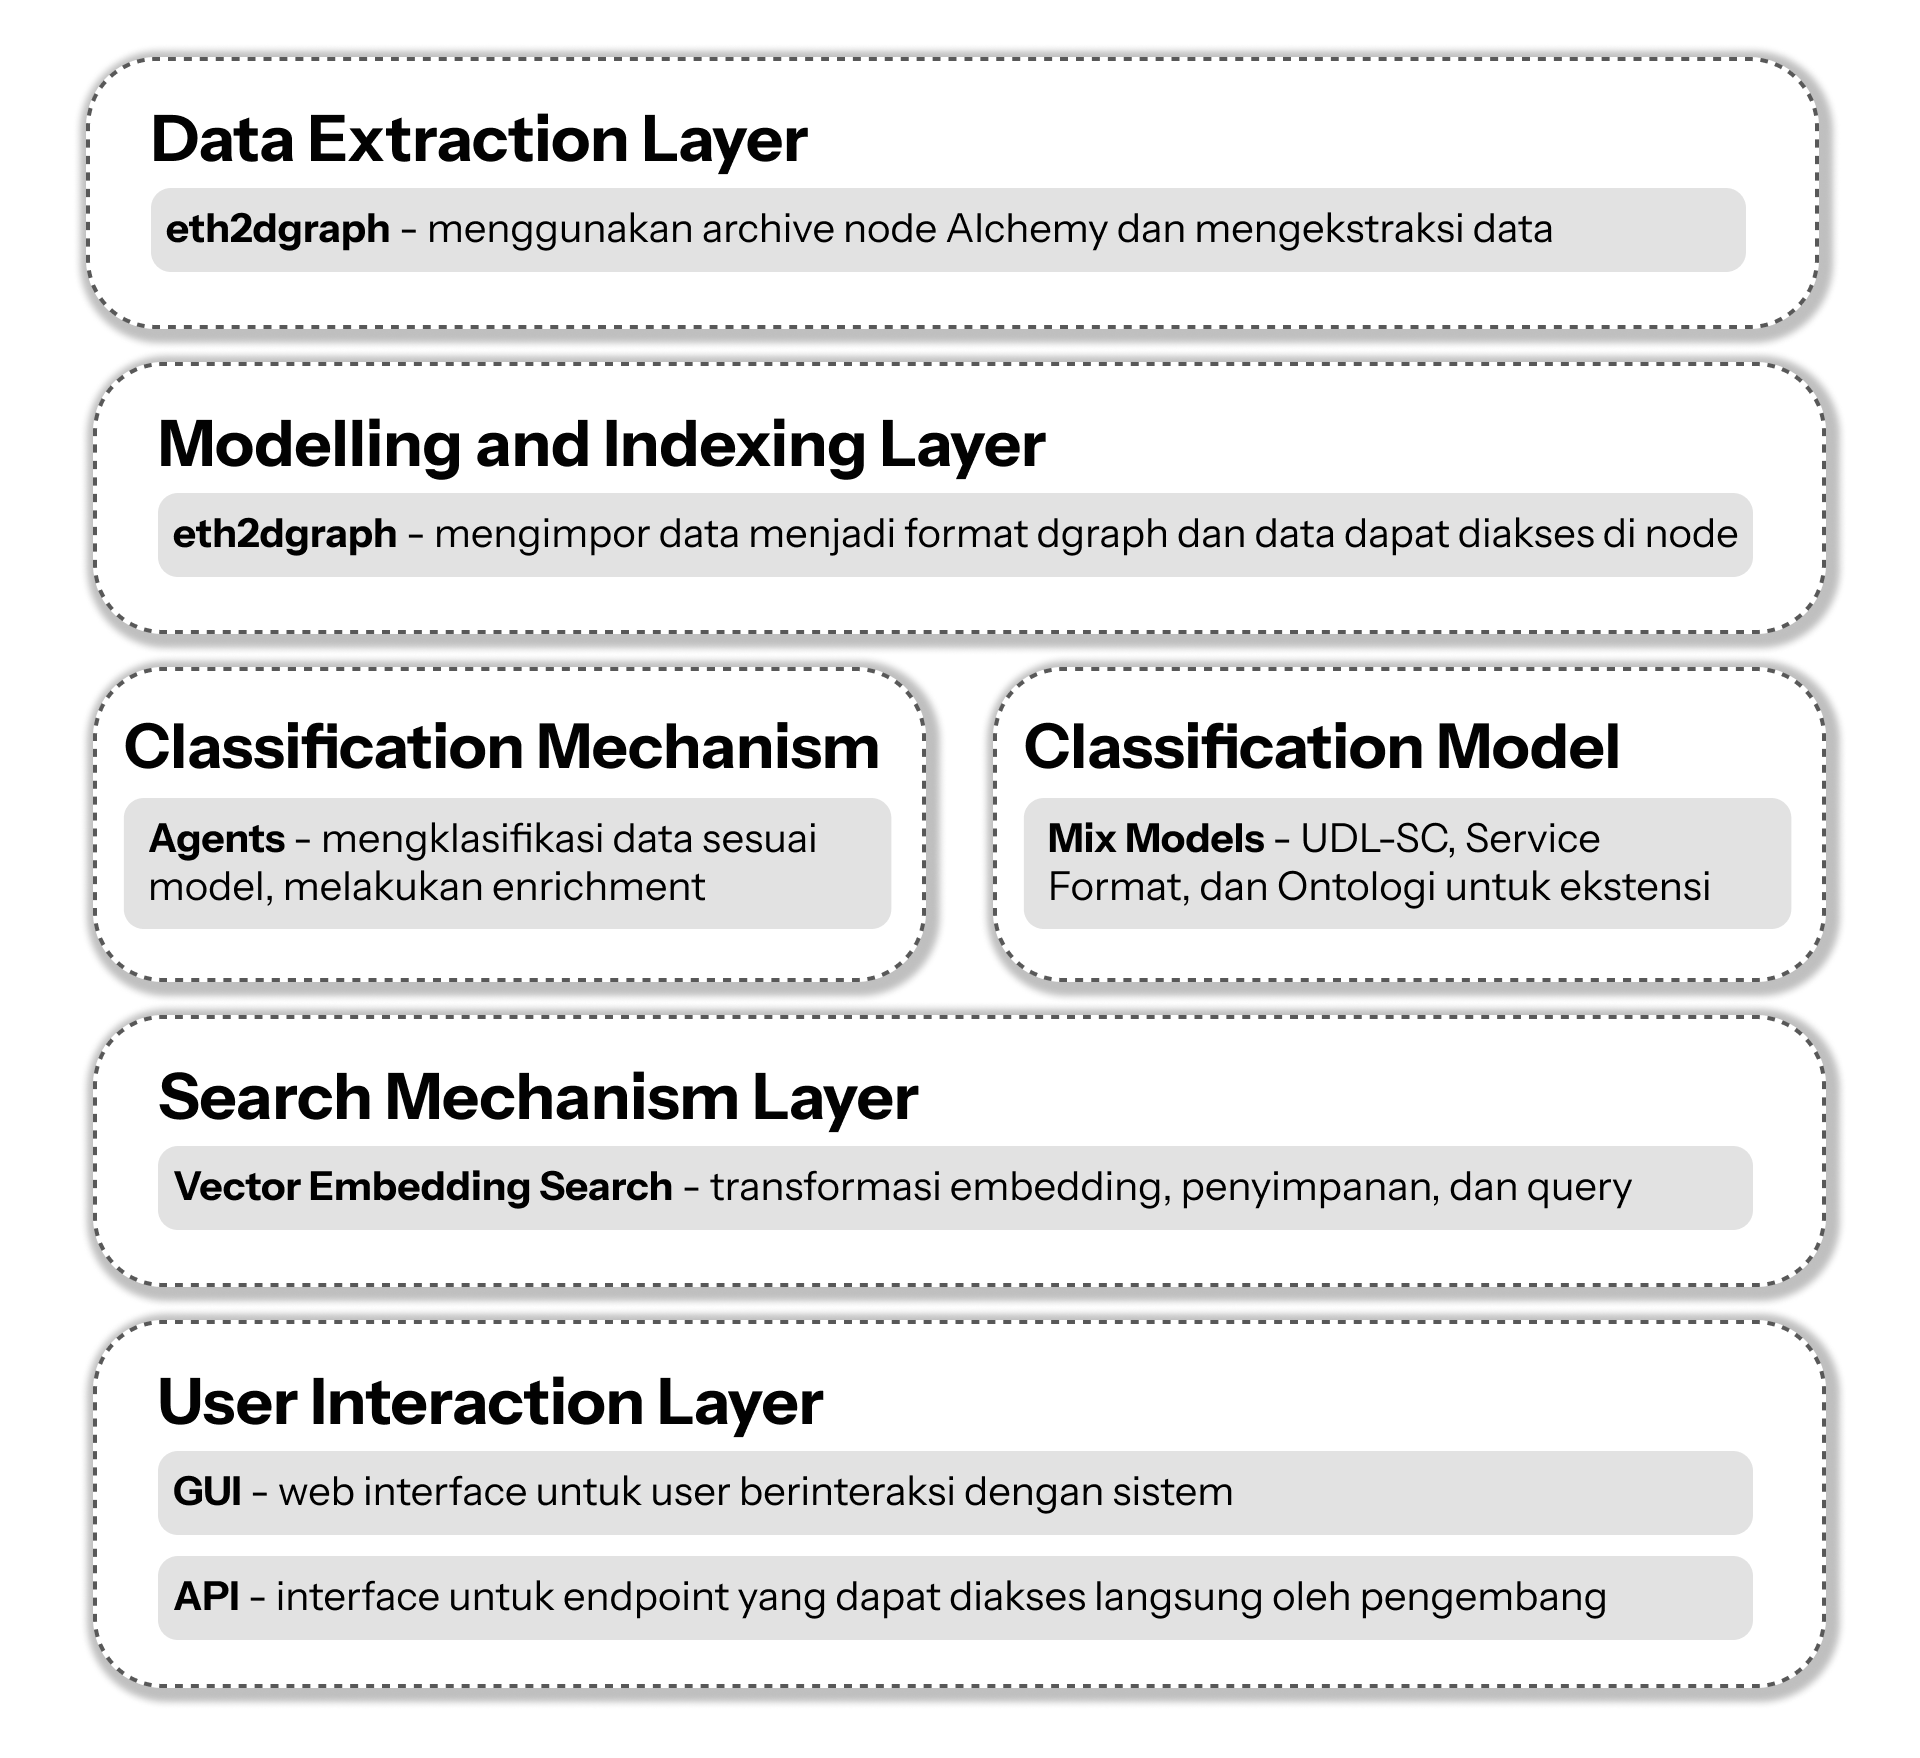
\includegraphics[width=0.7\textwidth]{resources/chapter-3/hasil-pemilihan.png}
	\caption{Kesimpulan pemilihan alternatif}
	\label{image:layer-architecture}
\end{figure}

Berdasarkan analisis dari alternatif-alternatif yang dibahas pada bagian \ref{subsec:analisis-alternatif-solusi}, dapat disimpulkan bahwa alternatif yang dipilih untuk membangun sistem adalah sebagai berikut:

\begin{enumerate}
	\item \textbf{Ekstraksi data Smart Contracts dari Blockchain Ethereum}: Alternatif yang dipilih adalah \textit{eth2dgraph} \parencite{aimar2023extraction}, karena memiliki aksesibilitas yang baik, bersifat \textit{open source}, memiliki kecepatan ekstraksi yang tinggi, dan juga menyediakan infrastruktur lengkap sampai pada penyimpanan data dalam format Distributed Graph Database.
	\item \textbf{Pemodelan, penyimpanan, dan \textit{indexing} data Smart Contracts}: Alternatif yang dipilih adalah \textit{eth2dgraph} \parencite{aimar2023extraction}, karena memiliki kemampuan skalabilitas tinggi dan dapat melakukan query dengan efisien. Selain itu, Dgraph juga memiliki kemampuan untuk melakukan \textit{indexing} data dengan baik.
	\item \textbf{Klasifikasi fungsional dan semantik Smart Contracts}: Alternatif yang dipilih untuk mekanisme klasifikasi adalah LLM Classification, karena memliki kemampuan kustomisasi yang baik untuk mendeskripsikan dan mengklasifikasi Smart Contracts. Model yang akan digunakan adalah model tekstual, yaitu penjelasan fungsionalitas Smart Contracts dalam bahasa alami, dengan kombinasi dengan konsep ontologi dalam bentuk metadata untuk pengklasifikasian. Metadata dengan konsep ontologi ini akan membuat atribut data lebih mudah untuk diekstrak menjadi sebuah ontologi.
	\item \textbf{Pencarian dan rekomendasi Smart Contracts}: Alternatif yang dipilih untuk mekanisme pencarian awal adalah alternatif Vector Embedding Search, karena simplisitas yang ditawarkan dan tidak ada redundansi \textit{layer}. Alternatif yang dapat dikonsiderasikan untuk pengembangan berikutnya, terutama jika dikembangkan sebuah fitur untuk berinteraksi dengan sistem yang lebih kompleks adalah alternatif \textit{Retrieval-Augmented Generation (RAG)}, karena dapat mengakomodasi interaksi yang lebih kompleks.
	\item \textbf{Interaksi pengguna dengan sistem}: API dan GUI akan diimplementasikan untuk interaksi pengguna dengan sistem karena dapat memberikan fleksibilitas dan kemudahan bagi pengguna. Sehingga, pengguna dapat melakukan pencarian Smart Contracts dengan cara yang sesuai dengan kebutuhan mereka.
\end{enumerate}

% Untuk mengatasi permasalahan pemilihan Smart Contracts yang tepat dan mengurangi redundansi Smart Contracts di Blockchain, solusi yang diusulkan adalah sebuah sistem pencarian Smart Contracts yang dapat memberikan hasil berdasarkan fungsionalitas Smart Contracts. Sistem akan dibangun dengan memanfaatkan berbagai teknologi dan riset yang sudah ada, yang melakukan \textit{indexing} maupun modeling yang menjadikan Smart Contracts \textit{discoverable} untuk mengefisiensikan pengembangan.

% Beberapa riset yang dilakukan peninjauan untuk digunakan sebagai basis adalah riset oleh \cite{third2017linked}, \cite{aimar2023extraction}, \cite{baqa2019semantic}, \cite{cano2021toward}. Peninjauan didasari dengan beberapa aspek yaitu aksesibilitas dari hasil riset, kompleksitas teknis, skalabilitas, dan dukungan fungsional untuk mencapai tujuan utama.

% % Masukin diagram yang dibuat di ppt

% % preliminary analysis

% % gambaran solusi

% % menjelaskan secara lebih detail latar belakang dan masalah yang menjadi dasar munculnya topik TA ini, intinya kita coba lihat & analisis gapnya 
% % gap analysis
% % kaitan antara sistem yang dikembangkan dengan yang terkait -> apa kelebihannya? atau apa kekurangan dari aplikasi lain? emang belum terpenuhi? apa yang belum terpenuhi?
% % posisi sistem yang dikembangkan terhadap sistem yang lebih besar

% % PLACEHOLDER
% \subsubsection{Semantic Indexing with Linked Data \parencite{third2017linked}}

% Riset ini menerapkan indeks semantik pada data Blockchain menggunakan Linked Data dengan keunggulan penggunaan ontology BLONDiE dan MSM untuk mendeskripsikan semantik Smart Contracts dan fokus pada aspek \textit{discoverability}. Secara aksesibilitas, konsep riset ini \textit{public}, namun tanpa implementasi \textit{open source}. Implementasinya kompleks karena memerlukan pemetaan ontology ekstensif dan RDF triple generation, tanpa dukungan \textit{tools} atau \textit{framework}. Skalabilitas riset ini terbatas karena bergantung pada RDF-based Linked Data, yang kurang cocok untuk data Blockchain besar.

% \subsubsection{eth2dgraph \parencite{aimar2023extraction}}

% Riset ini berfokus pada ekstraksi, \textit{indexing}, dan penyimpanan data Ethereum berbasis Distributed Graph. Keunggulannya adalah penggunaan ekstraksi ABI, bytecode, dan metadata yang dapat diubah menjadi format berbasis graf, serta implementasinya yang \textit{open source} dan \textit{public}. Menggunakan Rust untuk performa tinggi dan Dgraph untuk skalabilitas, riset ini dapat melakukan query pada hubungan Smart Contracts di Ethereum. Kompleksitasnya moderat karena memerlukan pengetahuan dasar tentang Rust dan Dgraph, namun dapat diperluas untuk menambahkan aspek semantik. Skalabilitasnya tinggi berkat kinerja Dgraph.

% \subsubsection{Alternatif Lainnya}

% Kedua riset alternatif lainnya oleh \cite{baqa2019semantic} dan \cite{cano2021toward} tidak dapat dipilih karena \textit{domain} yang terlalu spesifik, ditambah dengan implementasi yang tidak bersifat \textit{open source} dan \textit{public}.

% \subsubsection{Hasil Analisis}

% Setelah melakukan analisis dari alternatif yang ada, diputuskan untuk menggunakan riset oleh \cite{aimar2023extraction}, karena memiliki implementasi yang \textit{open source}, yang mempermudah ekstraksi dan \textit{indexing} data menjadi Graph Database, sehingga tidak perlu membuat RDF Triples ada model ontology dari awal. Distributed Graph Database juga memiliki skalabilitas yang baik untuk data yang banyak pada Blockchain Ethereum. eth2dgraph juga memiliki kemampuan ekstensibilitas yang baik dalam \textit{domain} yang lebih umum, sehingga lebih mudah diimplementasikan sebagai fondasi dari sistem keseluruhan. 

% \subsubsection{Rancangan Solusi}

% Dengan penggunaan eth2dgraph sebagai fondasi dari sistem pencarian Smart Contract, berikut merupakan ajuan rancangan dari sistem:

% \begin{enumerate}
%   \item Layer 1: Blockchain Data Extraction (eth2dgraph) \newline Ekstraksi data Blockchain Ethereum menjadi Dgraph
%   \item Layer 2: Semantic Indexing and Enrichment \newline \textit{Mapping} data hasil ekstraksi kepada sebuah ontology seperti BLONDiE atau EthOn, pelabelan fungsional Smart Contracts, dan Version Control
%   \item Layer 3: Query and Discovery System \newline Sebuah Search Engine menggunakan GraphQL Queries diatas Dgraph Database yang memperkenalkan pencarian berbasis semantik
%   \item Layer 4: User Interaction Layer \newline Sebuah \textit{dashboard} atau API untuk pengembang melakukan pencarian Smart Contracts berdasarkan fungsionalitas, metadata, atau relasi, membandingkan Smart Contracts yang serupa, dan melakukan \textit{export} atau \textit{reuse} dari Smart Contract 
% \end{enumerate}


\subsection{Analisis Kebutuhan Sistem}

% bingung nulis apa lagi disini
Pada bagian \ref{subsec:analisis-alternatif-solusi}, telah disimpulkan pilihan alternatif yang akan digunakan dalam membangun sistem. Alternatif-alternatif solusi yang digunakan akan menjadi komponen yang saling berinteraksi dalam sistem Smart Contract Discovery untuk menyediakan fungsionalitas yang terpadu. Pada bagian ini akan diuraikan lebih lanjut mengenai sistem yang akan dibangun sehingga dapat memberikan panduan dalam fase pengembangan sistem. Penjelasan ini mencakup deskripsi sistem, karakteristik pengguna, kebutuhan fungsional dan non-fungsional, serta model use case yang akan digunakan dalam sistem.

\subsubsection{Deskripsi Sistem}
% penjelasan gambaran umum sistem, komponen utamanya apa aja
% buat diagram UML gambaran umum
% Jelaskan tujuan utama sistem (misalnya: "Membangun sistem pencarian smart contract berbasis semantik untuk meningkatkan efisiensi pengembangan dApps").

Solusi yang akan dikembangkan adalah sebuah sistem Smart Contract Discovery yang bertujuan untuk menyediakan \textit{platform} pencarian Smart Contract dalam Blockchain Ethereum berbasis semantik memanfaatkan LLM dan RAG. Sistem akan dibagi menjadi beberapa komponen utama yang saling berinteraksi untuk menyediakan fungsionalitas yang terpadu. Komponen utama sistem adalah sebagai berikut:

\begin{enumerate}
  \item Komponen Ekstraksi Data
  \item Komponen Penyimpanan Data
  \item Komponen \textit{Semantic Enrichment}
  \item Komponen Pencarian
  \item Komponen Antarmuka Pengguna
\end{enumerate}

\begin{figure}[ht]
	\centering
	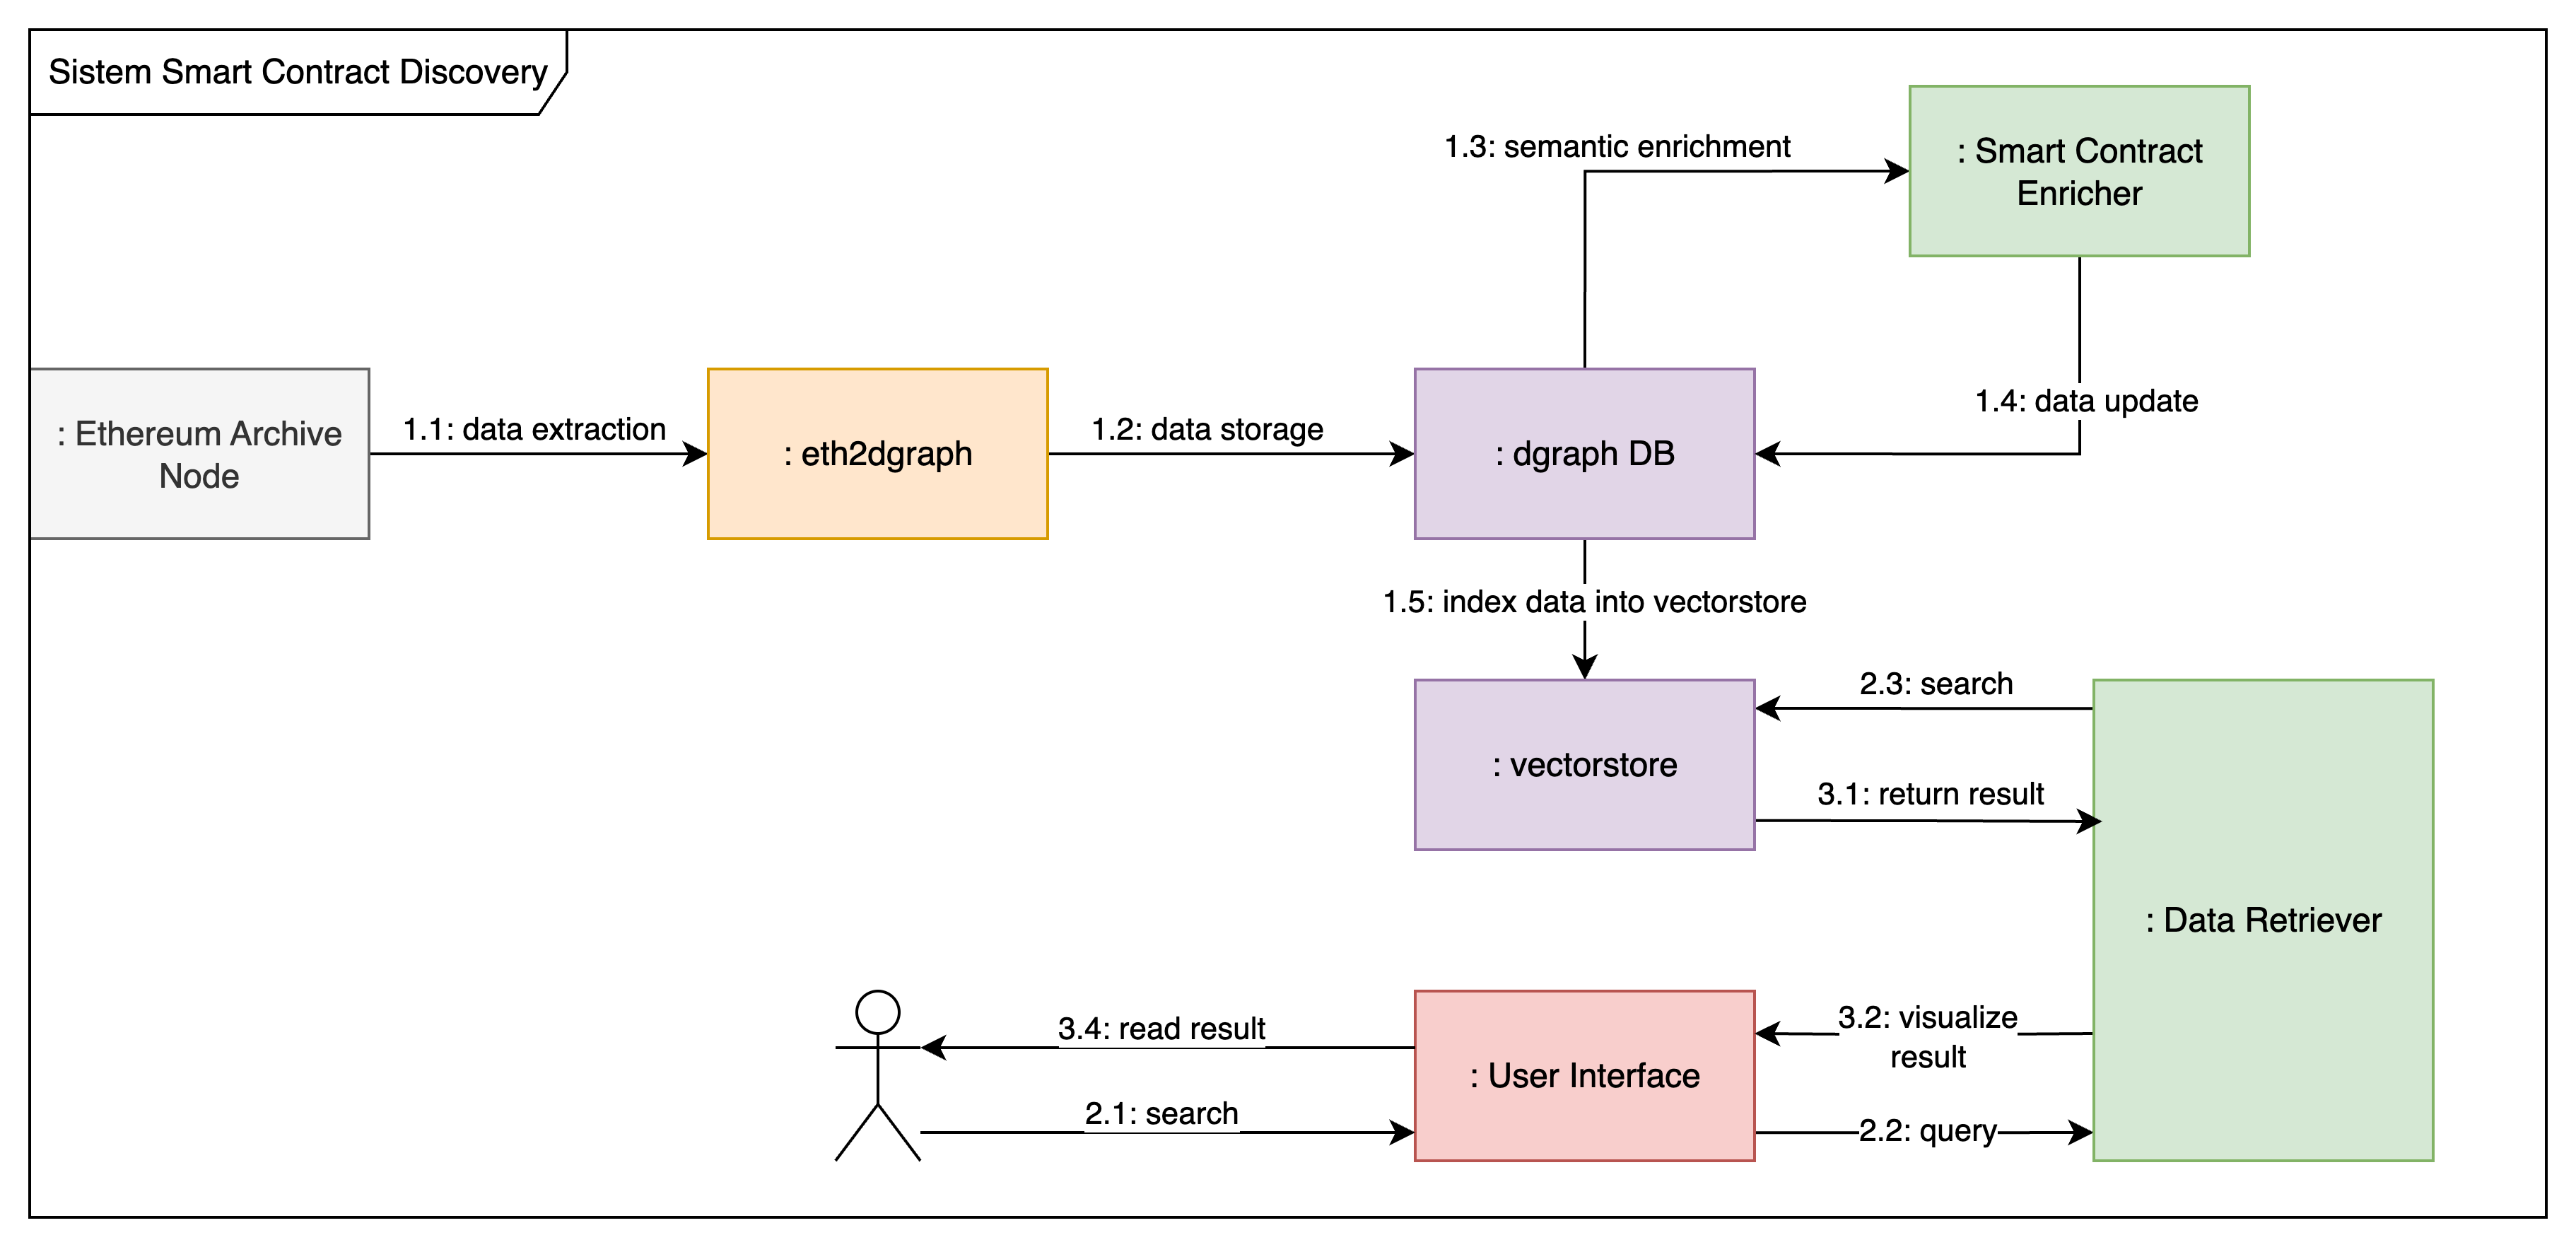
\includegraphics[width=1\textwidth]{resources/chapter-3/komponen-utama-new.png}
	\caption{Gambaran Umum Interaksi Komponen Utama Sistem}
	\label{image:komponen-sistem}
\end{figure}

\begin{figure}[ht]
	\centering
	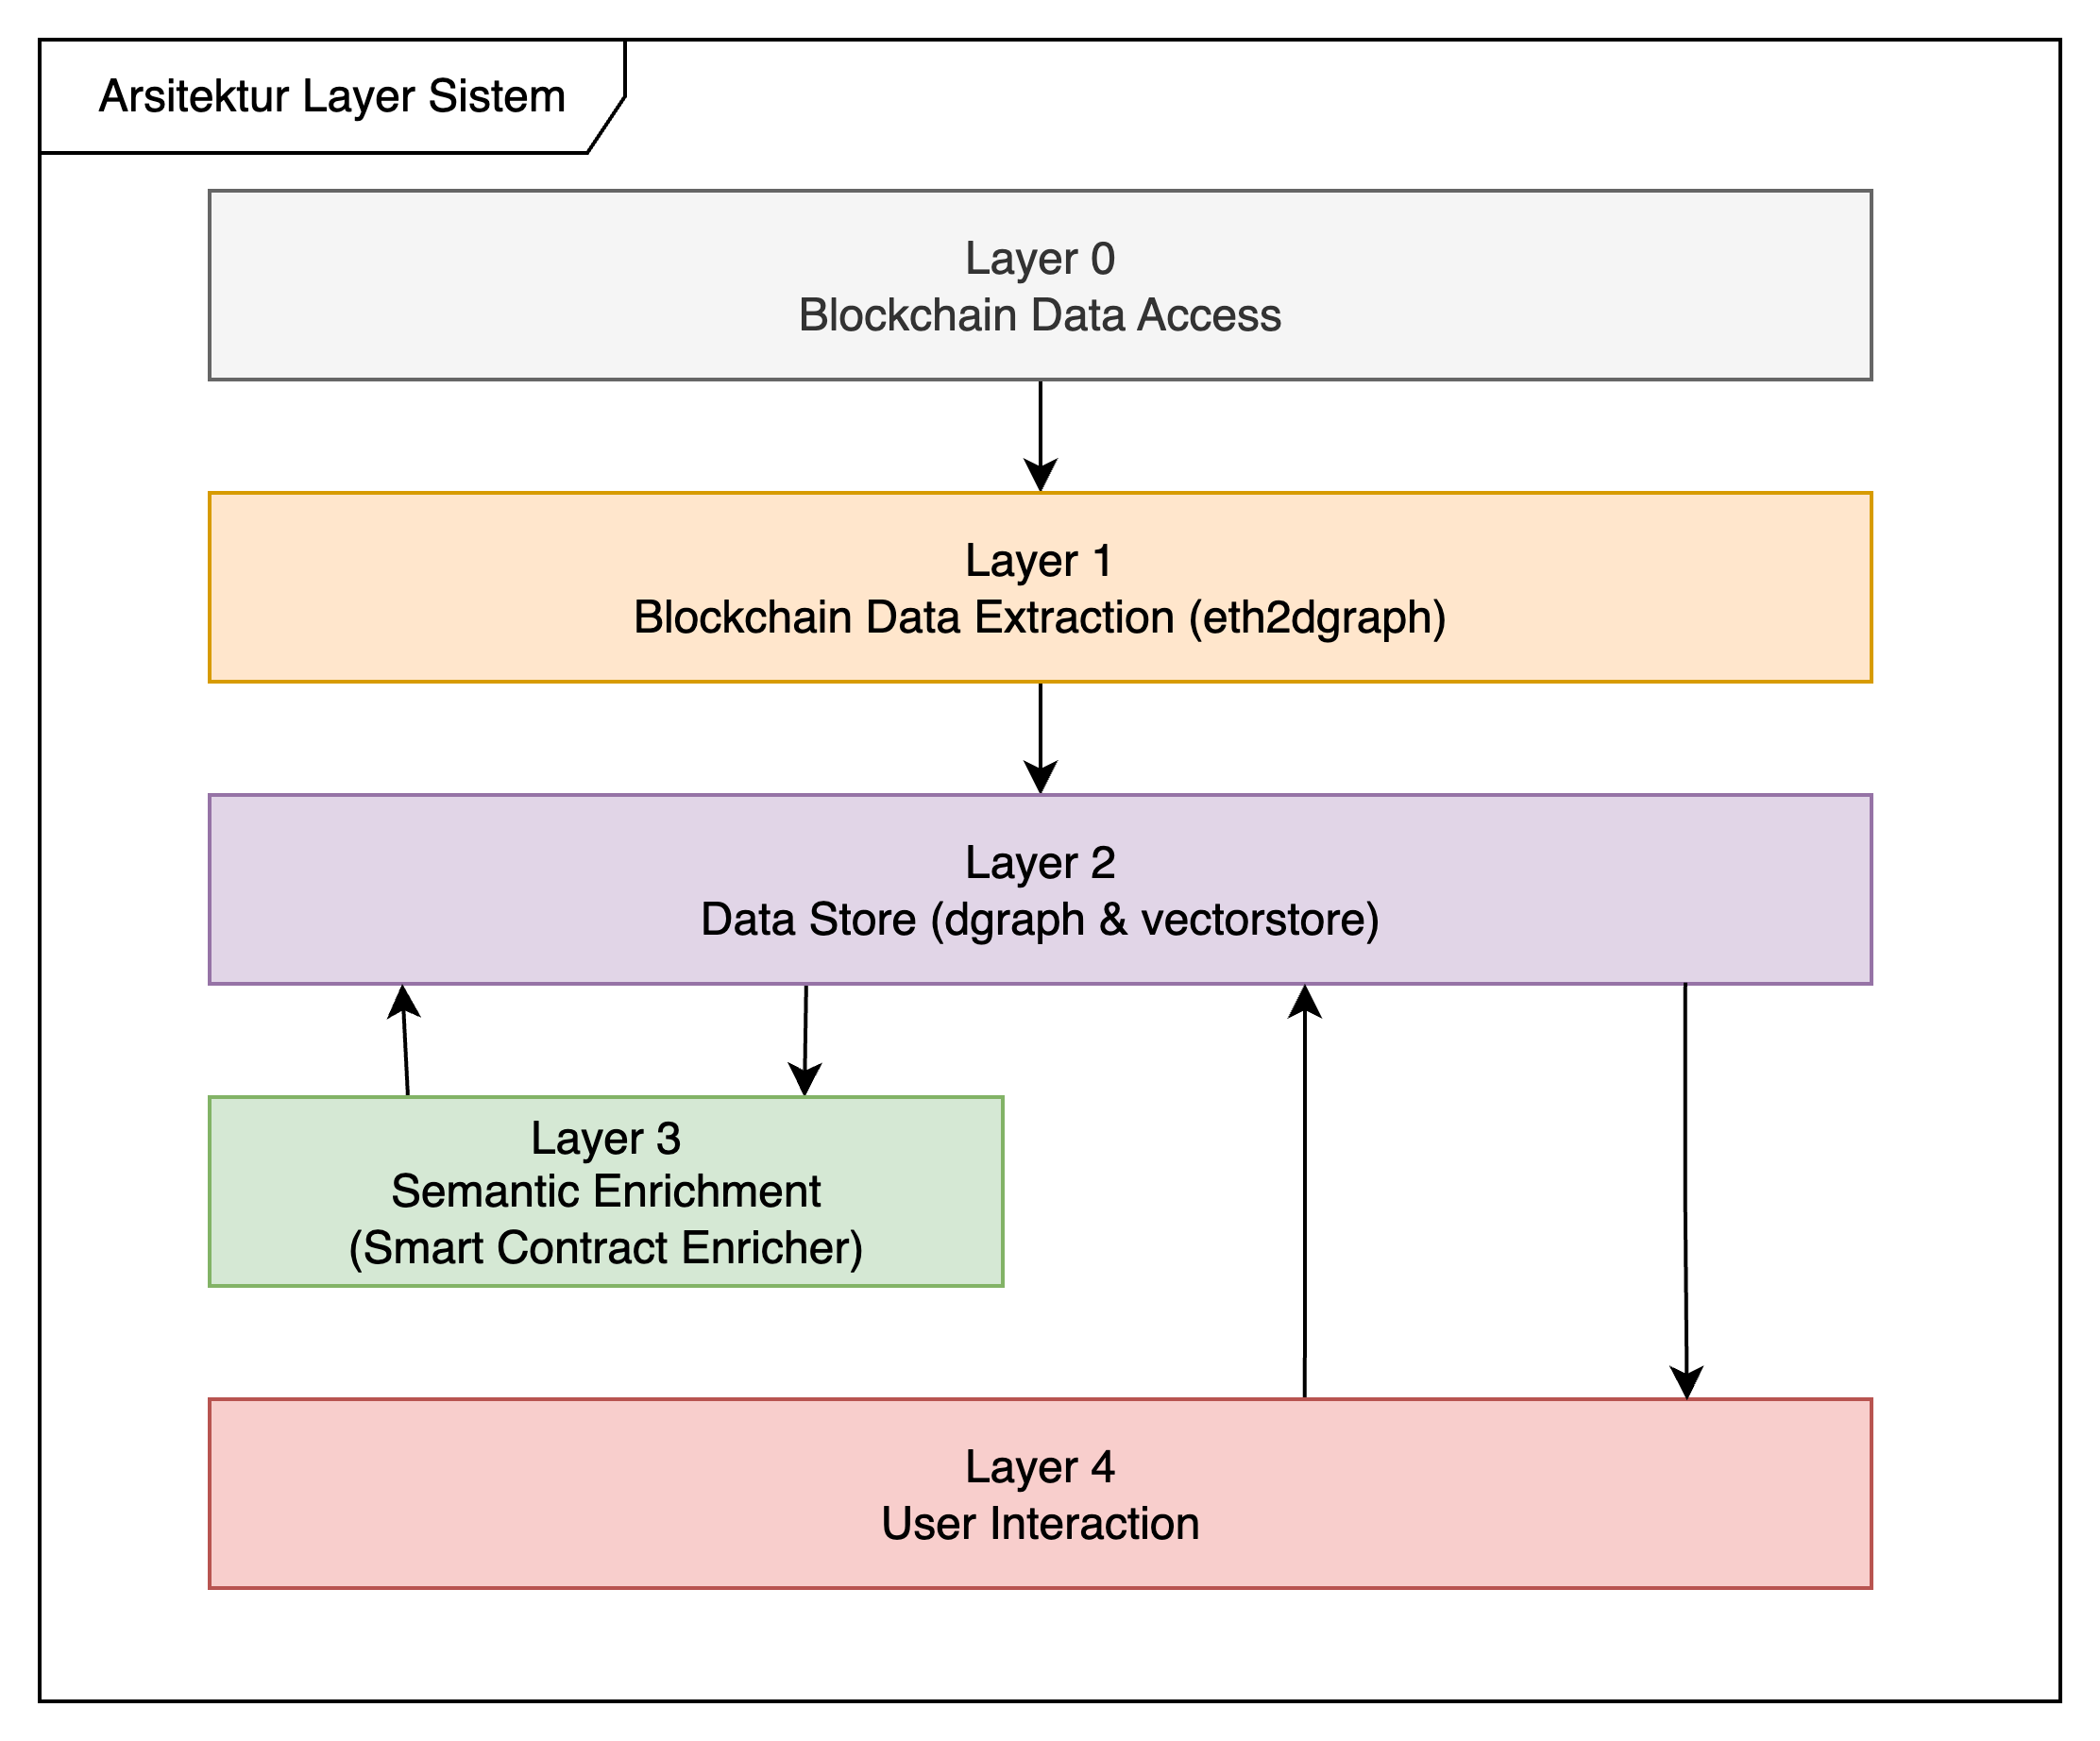
\includegraphics[width=0.7\textwidth]{resources/chapter-3/layer-arsitektur-new.png}
	\caption{Gambaran Arsitektur Layer Sistem}
	\label{image:layer-arsitektur}
\end{figure}

% Ethereum Archive Node → eth2dgraph (ekstraksi) → Dgraph (penyimpanan) → LLM (semantic enrichment) → Dgraph (update) → RAG (query).  

Gambar \ref{image:komponen-sistem} dan gambar \ref{image:layer-arsitektur} menunjukkan gambaran umum alur kerja sistem. Sistem ini akan melakukan ekstraksi data dari Ethereum Archive Node menggunakan \textit{eth2dgraph} dan menyimpannya dalam Dgraph. Setelah itu, sistem akan melakukan \textit{semantic enrichment} menggunakan LLM untuk memperkaya deskripsi dan metadata Smart Contract, lalu memperbarui data di Dgraph. Sebelum data dapat dilakukan query menggunakan RAG, akan dilakukan indexing data menjadi bentuk vectorstore. Terakhir, sistem akan menggunakan RAG untuk melakukan pencarian berdasarkan kebutuhan pengguna. 



\subsubsection{Karakteristik Pengguna}

Sistem ini hanya akan digunakan oleh satu jenis pengguna, yaitu User yang ingin mencari Smart Contract. Belum ada mekanisme yang membutuhkan campur tangan pengguna lain, seperti pengembang atau administrator. Pengguna dapat melakukan pencarian Smart Contract berdasarkan kebutuhan fungsionalitas yang diinginkan. Pengguna tidak perlu memiliki pengetahuan teknis yang mendalam tentang Smart Contract atau Blockchain untuk menggunakan sistem ini. Antarmuka pengguna dirancang agar mudah digunakan dan intuitif, sehingga pengguna dapat dengan mudah menemukan Smart Contract yang sesuai dengan kebutuhan mereka, dan menggunakannya, baik digunakan secara langsung, atau menjadi komponen di dalam aplikasi yang lebih besar.

\subsubsection{Kebutuhan Fungsional}

Sistem ini memiliki beberapa kebutuhan fungsional yang harus dipenuhi agar dapat berfungsi dengan baik. Kebutuhan fungsional ini mencakup semua fitur dan fungsi yang harus ada dalam sistem untuk memenuhi tujuan utama sistem. Berikut adalah daftar kebutuhan fungsional yang diidentifikasi:

% tabel
% \begin{table}[h]
% 	\caption{Kebutuhan Fungsional Sistem}
% 	\vspace{0.25cm}
% 	\begin{center}
% 		\begin{tabular}{|c|l|}
% 			\hline
% 			\textbf{ID} & \textbf{Penjelasan} \\ \hline
% 			F01 & User dapat melakukan input kebutuhan dalam bentuk \textit{Natural Language} \\ \hline
% 			F02 & User dapat mencari Smart Contract  \\ \hline
% 			F03 & Pengembangan Prototipe \\ \hline
% 			F04 & Pengujian Prototipe \\ \hline
% 			F05 & Evaluasi dan Perbaikan \\ \hline
% 		\end{tabular}
% 	\end{center}
% \end{table}

\subsubsection{Kebutuhan Non-Fungsional}

\subsubsection{Model Use Case}

Kebutuhan fungsional dan karakteristik pengguna yang dirumuskan dapat dimodelkan menjadi use case. Seperti pada gambar \ref{image:usecase}, Use case kemudian dapat dipetakan menjadi sebuah Use Case Diagram yang menghubungkan relasi antara aktor dengan use case yang berkolerasi. Diagram ini menggambarkan interaksi antara pengguna dan sistem, serta fungsi-fungsi yang tersedia dalam sistem. Diagram use case ini akan membantu dalam memahami bagaimana pengguna akan berinteraksi dengan sistem dan fitur-fitur apa saja yang harus ada dalam sistem. Use case dapat dilihat secara detail pada lampiran XX.

\begin{figure}[ht]
	\centering
	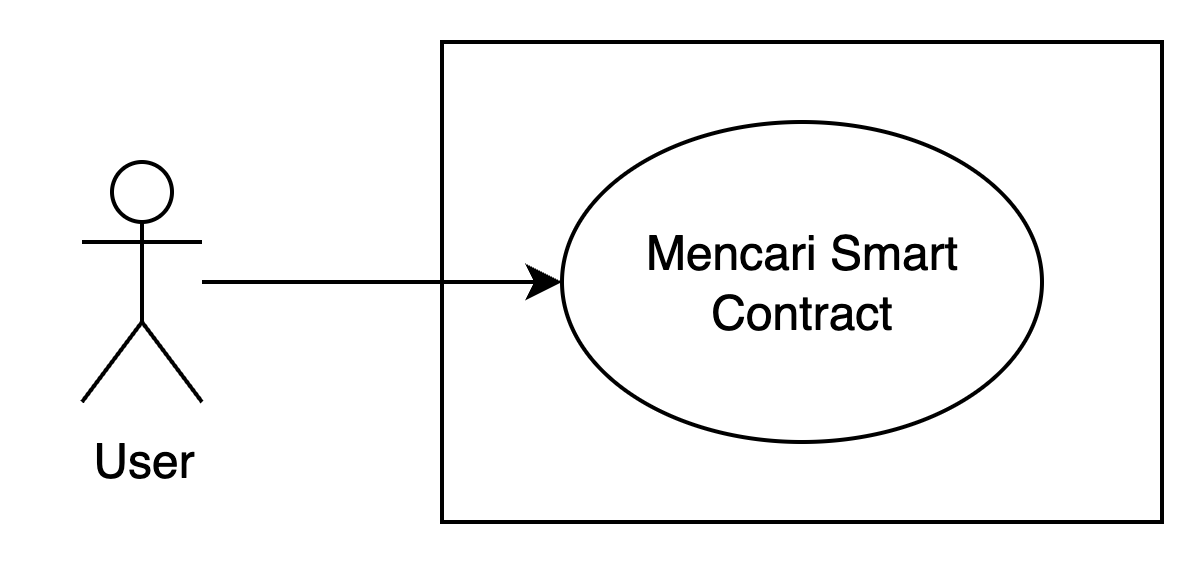
\includegraphics[width=0.7\textwidth]{resources/chapter-3/use-case.png}
	\caption{Use Case Diagram}
	\label{image:usecase}
\end{figure}

\subsubsection{Risiko dan Mitigasi}


\break

\section{Rancangan}

